\documentclass[11pt,a4paper]{article}

% Image mode: pdf.
% Image paths stay relative. In PDF mode, place same-basename PDF conversions
% of the chapter SVG files in the assets/ directory beside this source.

\usepackage{iftex}
\ifPDFTeX
  \PackageError{handout}{This template requires XeTeX or Tectonic}{Compile with xelatex or tectonic.}
\fi

\usepackage[a4paper,top=18mm,bottom=20mm,left=20mm,right=20mm,headsep=6mm]{geometry}
\usepackage{fontspec}
\usepackage{xeCJK}
\usepackage{amsmath}
\usepackage{unicode-math}

% Font settings are intentionally visible in the generated .tex file.
% These defaults target the macOS machine used for the released PDF.
% Change the family names when compiling on another system.
\setmainfont{Songti TC}
\setsansfont{Heiti TC}
\setmonofont{Menlo}
\setCJKmainfont{Songti TC}
\setCJKsansfont{Heiti TC}
\setCJKmonofont{Heiti TC}
\setmathfont{STIX Two Math}
\XeTeXlinebreaklocale "zh"
\XeTeXlinebreakskip=0pt plus 1pt

\usepackage{xcolor}
\definecolor{HandoutBlue}{HTML}{215A91}
\definecolor{HandoutBlueLight}{HTML}{EEF5FC}
\definecolor{HandoutGreen}{HTML}{39715A}
\definecolor{HandoutGreenLight}{HTML}{EFF8F3}
\definecolor{HandoutGold}{HTML}{8A641C}
\definecolor{HandoutGoldLight}{HTML}{FFF8E8}
\definecolor{HandoutInk}{HTML}{253142}
\definecolor{HandoutMuted}{HTML}{667085}

\usepackage{graphicx}
\makeatletter
% Pandoc 3 emits an accessibility `alt` key for raster/PDF images. Older
% graphicx releases do not know that key, so accept it without changing layout.
\@ifundefined{KV@Gin@alt}{\define@key{Gin}{alt}{}}{}
\newsavebox\pandoc@box
\newcommand*\pandocbounded[1]{%
  \sbox\pandoc@box{#1}%
  \Gscale@div\@tempa{\textheight}{\dimexpr\ht\pandoc@box+\dp\pandoc@box\relax}%
  \Gscale@div\@tempb{\linewidth}{\wd\pandoc@box}%
  \ifdim\@tempb\p@<\@tempa\p@\let\@tempa\@tempb\fi
  \ifdim\@tempa\p@<\p@\scalebox{\@tempa}{\usebox\pandoc@box}%
  \else\usebox{\pandoc@box}%
  \fi
}
\makeatother
\usepackage{float}
\floatplacement{figure}{H}
% Pandoc uses LTcaptype=none for uncaptioned longtables. The caption package
% expects that name to exist as a counter even though it is never displayed.
\newcounter{none}
\usepackage{caption}
\captionsetup[figure]{labelformat=empty,labelsep=none,font=small}

\usepackage{booktabs,longtable,array,calc}
\usepackage{etoolbox}
\makeatletter
\patchcmd\longtable{\par}{\if@noskipsec\mbox{}\fi\par}{}{}
\makeatother

\usepackage[most]{tcolorbox}
\tcbuselibrary{breakable,skins}
\newtcolorbox{HandoutLearningMap}{
  enhanced,breakable,colback=HandoutBlueLight,colframe=HandoutBlue,
  boxrule=0.8pt,arc=1.5mm,left=3mm,right=3mm,top=2mm,bottom=2mm,
  before skip=8pt,after skip=10pt
}
\newtcolorbox{HandoutWorkedExample}{
  enhanced,breakable,colback=HandoutGreenLight,colframe=HandoutGreen,
  boxrule=0.65pt,arc=1.5mm,left=3mm,right=3mm,top=2mm,bottom=2mm,
  before skip=8pt,after skip=10pt
}
\newtcolorbox{HandoutSelfCheck}{
  enhanced,breakable,colback=HandoutGoldLight,colframe=HandoutGold,
  boxrule=0.65pt,arc=1.5mm,left=3mm,right=3mm,top=2mm,bottom=2mm,
  before skip=8pt,after skip=10pt
}

\usepackage{titlesec}
\titleformat{\section}{\sffamily\bfseries\Large\color{HandoutBlue}}{}{0pt}{}
\titleformat{\subsection}{\sffamily\bfseries\large\color{HandoutInk}}{}{0pt}{}
\titleformat{\subsubsection}{\sffamily\bfseries\normalsize\color{HandoutInk}}{}{0pt}{}
\titlespacing*{\section}{0pt}{1.4em}{0.55em}
\titlespacing*{\subsection}{0pt}{1.15em}{0.45em}
\titlespacing*{\subsubsection}{0pt}{0.9em}{0.35em}
\setcounter{secnumdepth}{-\maxdimen}

\usepackage{hyperref}
\usepackage{bookmark}
\IfFileExists{xurl.sty}{\usepackage{xurl}}{}
\urlstyle{same}
\hypersetup{
  colorlinks=true,
  linkcolor=HandoutBlue,
  urlcolor=HandoutBlue,
  citecolor=HandoutBlue,
  pdftitle={必化-3 溶液與常見的化學反應},
  pdfsubject={化學},
  pdfcreator={Pandoc with the HighSchooContent LaTeX template}
}

\setlength{\parindent}{0pt}
\setlength{\parskip}{0.55em plus 0.15em minus 0.1em}
\setlength{\emergencystretch}{3em}
\setlength{\LTpre}{0.5em}
\setlength{\LTpost}{0.5em}
\renewcommand{\arraystretch}{1.18}
\providecommand{\tightlist}{%
  \setlength{\itemsep}{0pt}\setlength{\parskip}{0pt}}
\pagestyle{plain}


\begin{document}

\begin{tcolorbox}[
  enhanced,colback=white,colframe=HandoutBlue,boxrule=1.1pt,arc=2mm,
  borderline west={3pt}{0pt}{HandoutBlue},left=5mm,right=4mm,top=4mm,bottom=4mm
]
{\sffamily\small\bfseries\color{HandoutBlue}學生講義}\par
{\sffamily\bfseries\LARGE\color{HandoutInk}必化-3 溶液與常見的化學反應}\par
\vspace{0.35em}{\large 由粒子分布與定量資料判斷溶液組成、溶解平衡、酸鹼與電子轉移}\par
\vspace{0.45em}{\small\color{HandoutMuted}%
科目：化學
\quad 課程：普通高中必修化學
\quad 版本：學生版｜核心＋理解
\quad 校訂：2026-08-29
}\par
\vspace{0.25em}{\small\color{HandoutMuted}範圍：現行必修化學第三章主線；含溶液與濃度、溶解度、酸鹼反應及氧化還原，亨利定律、極稀溶液修正與氧化數系統演算留待選修}\par
\end{tcolorbox}


溶液的外觀看來均勻，內部仍有持續運動的分子或離子。濃度把每單位溶液中的物質量化；溶解度指出固定條件下可達的上限；酸鹼反應追蹤 \(H^+\) 與 \(OH^-\)；氧化還原反應追蹤電子。實際應用包括配製標準溶液、處理水質資料、控制結晶純化、估算制酸劑用量、判讀金屬腐蝕與電池反應。

計算時先辨認資料的基準：分母是溶液質量、溶液體積，還是溶劑質量。反應題再把濃度換成莫耳數，依反應式決定消耗量與剩餘量。觀察只能提供證據；粒子種類與反應方向仍需由模型和守恆關係推論。

\textbf{核心問題：}如何用濃度描述溶液、如何由溶解度預測結晶、如何由 \(K_w\) 與化學計量判斷酸鹼，以及如何由電子得失辨認氧化劑和還原劑。

\section{1. 溶液、分散系、濃度與配製}\label{ux6eb6ux6db2ux5206ux6563ux7cfbux6fc3ux5ea6ux8207ux914dux88fd}

\subsection{1.1 溶液是均勻混合物}\label{ux6eb6ux6db2ux662fux5747ux52fbux6df7ux5408ux7269}

\textbf{溶液}是由兩種以上純物質形成的均勻混合物。通常含量較多、決定溶液物態的成分稱為\textbf{溶劑}，其餘成分稱為\textbf{溶質}；水溶液中的水一律視為溶劑。溶液可依物態分為氣態、液態與固態，例如空氣、食鹽水與黃銅。

溶於水後形成可移動離子的物質稱為\textbf{電解質}。NaCl 水溶液含 \(Na^+\) 與 \(Cl^-\)，可導電；蔗糖以中性分子分散，屬非電解質水溶液。導電性取決於可移動帶電粒子的種類與數量，不能只由物質是否含金屬元素判斷。

依分散粒子直徑可區分三種系統：

\begin{itemize}
\tightlist
\item
  \textbf{真溶液：}粒徑小於 \(1\ \mathrm{nm}\)，均勻且久置不沉降，通常看不到光束通過的路徑。
\item
  \textbf{膠體：}粒徑約 \(1\) 至 \(1000\ \mathrm{nm}\)，粒子散射可見光而形成\textbf{廷得耳效應}。
\item
  \textbf{懸浮液：}粒徑通常大於 \(1000\ \mathrm{nm}\)，久置會因重力而沉降，可由過濾等方法分離。
\end{itemize}

\begin{figure}
\centering
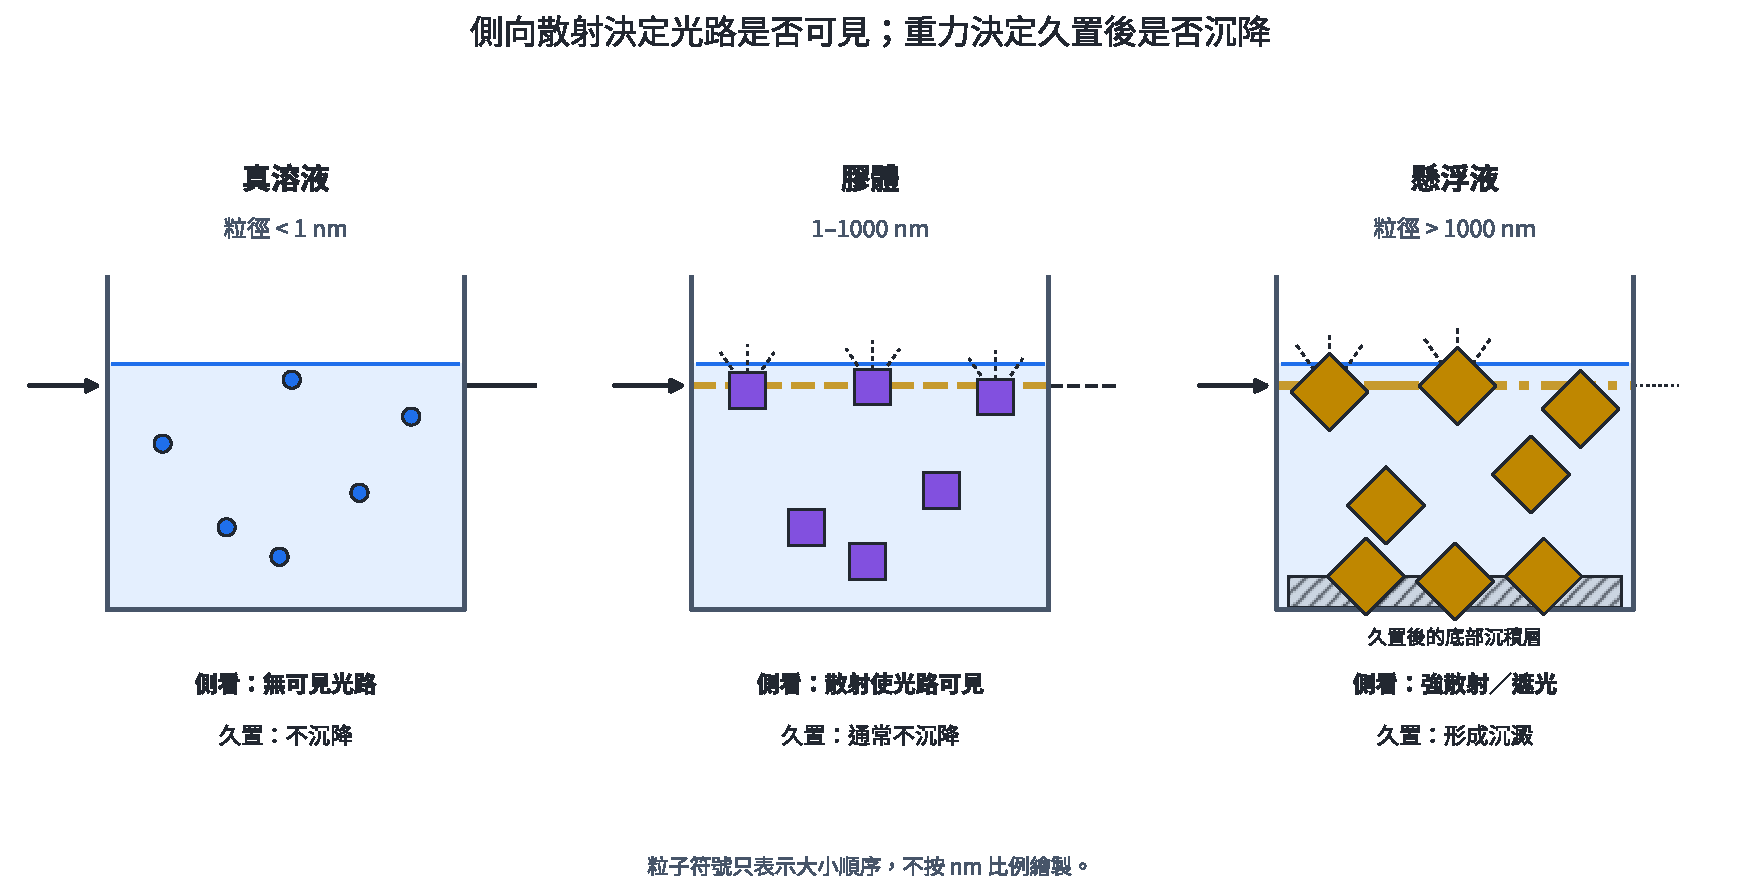
\includegraphics[width=0.98\linewidth,height=\textheight,keepaspectratio,alt={圖 1｜側向散射使膠體與懸浮液的光路可見；久置沉降再把懸浮液與膠體分開。粒子符號只表示大小順序。}]{assets/必化-3-分散粒徑與光路.pdf}
\caption{圖 1｜側向散射使膠體與懸浮液的光路可見；久置沉降再把懸浮液與膠體分開。粒子符號只表示大小順序。}
\end{figure}

廷得耳效應可用來分辨外觀透明的真溶液與膠體，例如霧、牛奶與某些奈米分散液。它只表示有足以散射光的粒子，不能直接指出粒子的化學成分。

\subsection{1.2 濃度必須連同分母一起讀}\label{ux6fc3ux5ea6ux5fc5ux9808ux9023ux540cux5206ux6bcdux4e00ux8d77ux8b80}

\textbf{濃度}表示一定量溶液或溶劑中含多少溶質。不同表示法回答不同問題。

\textbf{質量百分率濃度}以溶液質量為分母：

\[
w\%=\frac{m_{\mathrm{solute}}}{m_{\mathrm{solution}}}\times100\%.
\]

若把 \(20.0\ \mathrm g\) NaCl 與 \(80.0\ \mathrm g\) 水混合且完全溶解，溶液質量為 \(100.0\ \mathrm g\)，質量百分率為 \(20.0\%\)。溶劑質量不在這個公式的分母。

\textbf{百萬分點濃度}適合描述微量物質：

\[
C_{\mathrm{ppm}}
=\frac{m_{\mathrm{solute}}}{m_{\mathrm{solution}}}\times10^6.
\]

\(1\ \mathrm{ppm}\) 的質量意義是每 \(1\ \mathrm{kg}\) 溶液含 \(1\ \mathrm{mg}\) 溶質。極稀水溶液若密度接近 \(1.00\ \mathrm{kg\,L^{-1}}\)，才可近似寫成 \(1\ \mathrm{mg\,L^{-1}}\approx1\ \mathrm{ppm}\)。密度差異明顯時，需先把體積換成質量。

\textbf{體積莫耳濃度}或\textbf{莫耳濃度}以溶液體積為分母：

\[
C=\frac{n_{\mathrm{solute}}}{V_{\mathrm{solution}}},
\]

常用單位為 \(\mathrm{mol\,L^{-1}}\) 或 M。溶液體積會隨溫度改變，因此精密莫耳濃度需連同配製溫度與容量器材的校正條件理解。

同一溶液的質量百分率與莫耳濃度之間需要\textbf{密度}才能互換。以 \(100.0\ \mathrm g\) 溶液為基準時，先由百分率求溶質質量，再以密度求溶液體積：

\[
V_{\mathrm{solution}}=\frac{m_{\mathrm{solution}}}{\rho}.
\]

\subsection{1.3 定量配製與稀釋保存的是溶質莫耳數}\label{ux5b9aux91cfux914dux88fdux8207ux7a00ux91cbux4fddux5b58ux7684ux662fux6eb6ux8ceaux83abux8033ux6578}

由固體配製標準溶液時，先由 \(n=CV\) 求所需莫耳數，再由 \(m=nM\) 求質量。固體在燒杯中溶解後定量轉移至容量瓶，洗滌燒杯與玻棒的洗液也轉入；溶液回到室溫後加水至刻度，塞緊並倒轉混合。

\begin{figure}
\centering
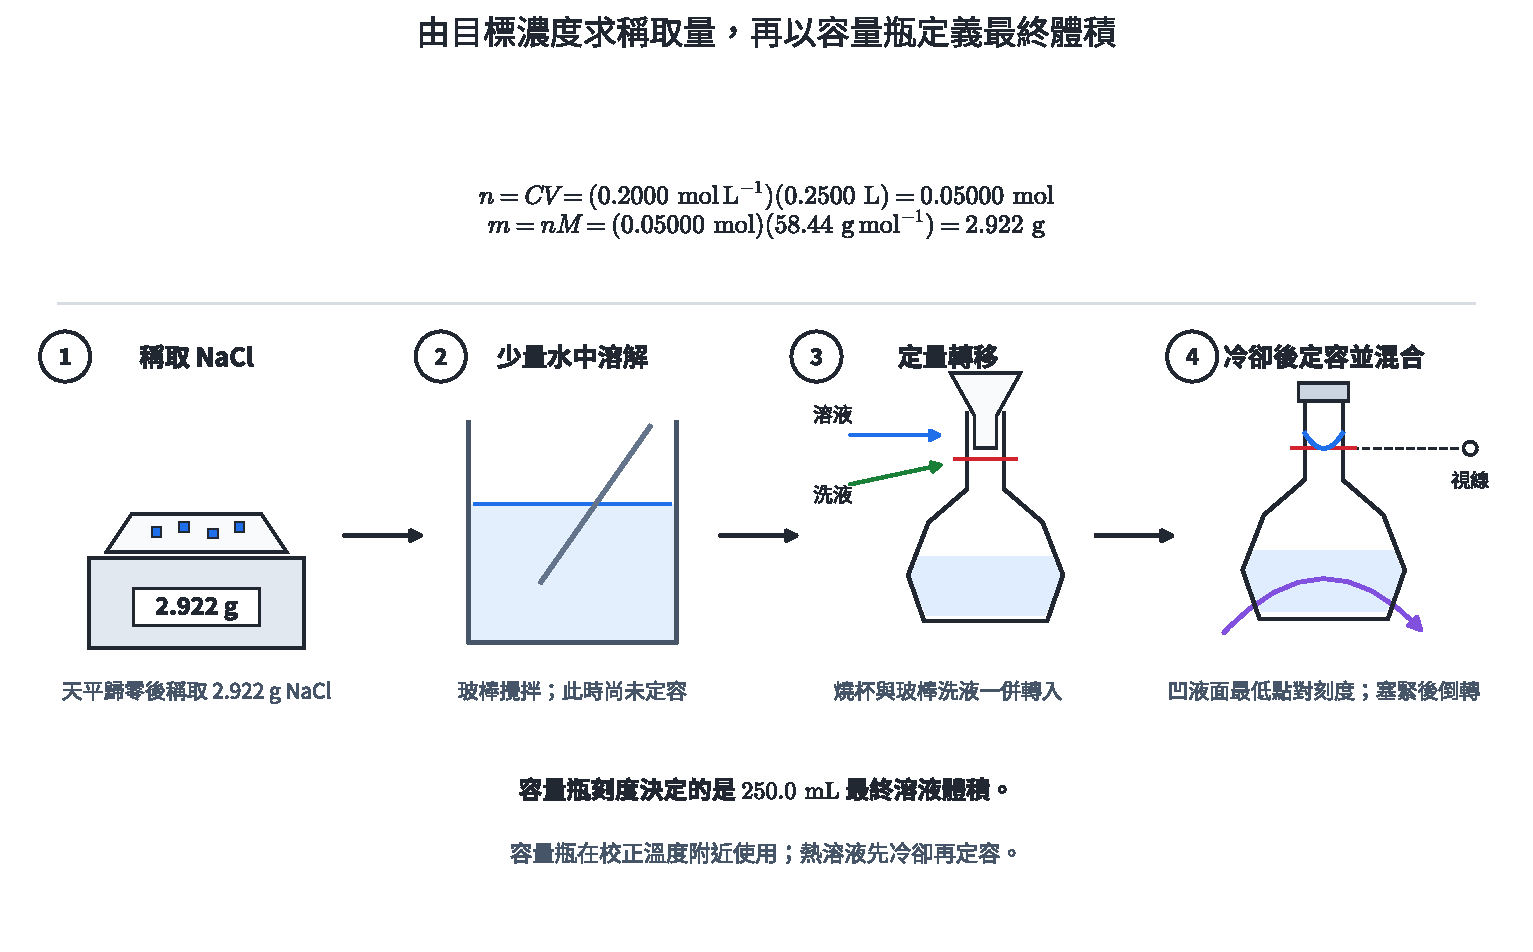
\includegraphics[width=0.98\linewidth,height=\textheight,keepaspectratio,alt={圖 2｜由 n=CV 求得配製 0.2000\textbackslash{} \textbackslash mathrm M NaCl 溶液需 2.922\textbackslash{} \textbackslash mathrm g NaCl；溶解、定量轉移與洗滌後，以凹液面最低點定容至 250.0\textbackslash{} \textbackslash mathrm\{mL\}。}]{assets/必化-3-濃度與定量配製.pdf}
\caption{圖 2｜由 \(n=CV\) 求得配製 \(0.2000\ \mathrm M\) NaCl 溶液需 \(2.922\ \mathrm g\) NaCl；溶解、定量轉移與洗滌後，以凹液面最低點定容至 \(250.0\ \mathrm{mL}\)。}
\end{figure}

取同一溶質的濃溶液加溶劑稀釋，若過程中沒有溶質損失或反應，稀釋前後溶質莫耳數相同：

\[
C_1V_1=C_2V_2.
\]

式中的 \(V_2\) 是稀釋後溶液的最終體積。液體混合時體積未必能直接相加，定量配製需以容量瓶刻度決定最終體積。

濃硫酸與水混合會大量放熱。實驗室稀釋時使用護目鏡、實驗衣與耐酸手套，在通風與冷卻條件下把酸沿器壁少量加入水並持續攪拌；含酸廢液依實驗室分類回收。若發生潑濺，立即依場域安全程序沖洗並通報。

\begin{HandoutWorkedExample}

\subsection{示範 1｜由粒徑與行為分類}\label{ux793aux7bc4-1ux7531ux7c92ux5f91ux8207ux884cux70baux5206ux985e}

三杯樣品分別是食鹽水、稀牛奶與泥水。雷射通過時，食鹽水看不到光路；稀牛奶可看到光路且久置不沉降；泥水久置有沉積。判斷三者。

食鹽水中的水合離子尺度小於 \(1\ \mathrm{nm}\)，屬真溶液。稀牛奶中的分散粒子能散射光且維持分散，屬膠體。泥水粒子久置沉降，屬懸浮液。分類依據是粒徑造成的光學與重力行為。

\end{HandoutWorkedExample}

\begin{HandoutWorkedExample}

\subsection{示範 2｜質量百分率與 ppm}\label{ux793aux7bc4-2ux8ceaux91cfux767eux5206ux7387ux8207-ppm}

將 \(8.00\ \mathrm g\) 葡萄糖溶於 \(192.00\ \mathrm g\) 水。求質量百分率；另有 \(2.50\ \mathrm{mg}\) 污染物存在於 \(1.25\ \mathrm{kg}\) 水樣中，求 ppm。

葡萄糖溶液總質量為

\[
8.00+192.00=200.00\ \mathrm g,
\]

故

\[
w\%=\frac{8.00}{200.00}\times100\%=4.00\%.
\]

水樣極稀，可把總質量視為 \(1.25\ \mathrm{kg}\)：

\[
C=\frac{2.50\ \mathrm{mg}}{1.25\ \mathrm{kg}}=2.00\ \mathrm{mg\,kg^{-1}}=2.00\ \mathrm{ppm}.
\]

\end{HandoutWorkedExample}

\begin{HandoutWorkedExample}

\subsection{示範 3｜溶質與離子的莫耳濃度}\label{ux793aux7bc4-3ux6eb6ux8ceaux8207ux96e2ux5b50ux7684ux83abux8033ux6fc3ux5ea6}

將 \(2.65\ \mathrm g\) 無水 \(Na_2CO_3\) 配成 \(250.0\ \mathrm{mL}\) 溶液。取 \(M(Na_2CO_3)=106.0\ \mathrm{g\,mol^{-1}}\)，求 \([Na_2CO_3]\)、\([Na^+]\) 與 \([CO_3^{2-}]\)。

\[
n(Na_2CO_3)=\frac{2.65}{106.0}=0.0250\ \mathrm{mol},
\]

\[
[Na_2CO_3]=\frac{0.0250}{0.2500}=0.100\ \mathrm M.
\]

由

\[
Na_2CO_3(aq)\rightarrow2Na^+(aq)+CO_3^{2-}(aq),
\]

可得

\[
[Na^+]=0.200\ \mathrm M,\qquad[CO_3^{2-}]=0.100\ \mathrm M.
\]

正電荷濃度為 \(0.200\ \mathrm{mol\,L^{-1}}\) 的單位正電荷，負電荷濃度為 \(0.100\times2=0.200\ \mathrm{mol\,L^{-1}}\) 的單位負電荷，符合電中性。

\end{HandoutWorkedExample}

\begin{HandoutWorkedExample}

\subsection{示範 4｜由質量百分率與密度求莫耳濃度}\label{ux793aux7bc4-4ux7531ux8ceaux91cfux767eux5206ux7387ux8207ux5bc6ux5ea6ux6c42ux83abux8033ux6fc3ux5ea6}

某 \(NaCl\) 水溶液的質量百分率為 \(12.0\%\)，密度為 \(1.08\ \mathrm{g\,mL^{-1}}\)。取 \(M(NaCl)=58.44\ \mathrm{g\,mol^{-1}}\)，求莫耳濃度。

以 \(100.0\ \mathrm g\) 溶液為基準，含 \(12.0\ \mathrm g\) NaCl：

\[
n=\frac{12.0}{58.44}=0.2053\ \mathrm{mol}.
\]

溶液體積為

\[
V=\frac{100.0\ \mathrm g}{1.08\ \mathrm{g\,mL^{-1}}}
=92.6\ \mathrm{mL}=0.0926\ \mathrm L.
\]

\[
C=\frac{0.2053}{0.0926}=2.22\ \mathrm M.
\]

\end{HandoutWorkedExample}

\begin{HandoutWorkedExample}

\subsection{示範 5｜由含結晶水固體配製溶液}\label{ux793aux7bc4-5ux7531ux542bux7d50ux6676ux6c34ux56faux9ad4ux914dux88fdux6eb6ux6db2}

用 \(CuSO_4\cdot5H_2O\) 配製 \(0.100\ \mathrm M\) 的 \(CuSO_4\) 水溶液 \(250.0\ \mathrm{mL}\)。取 \(M(CuSO_4\cdot5H_2O)=250.0\ \mathrm{g\,mol^{-1}}\)，求需稱取的質量。

每莫耳五水硫酸銅提供一莫耳 \(CuSO_4\)：

\[
n=CV=(0.100)(0.2500)=0.0250\ \mathrm{mol}.
\]

\[
m=(0.0250)(250.0)=6.25\ \mathrm g.
\]

稱量所用的莫耳質量必須對應實際試藥 \(CuSO_4\cdot5H_2O\)。

\end{HandoutWorkedExample}

\begin{HandoutWorkedExample}

\subsection{示範 6｜由濃溶液稀釋}\label{ux793aux7bc4-6ux7531ux6fc3ux6eb6ux6db2ux7a00ux91cb}

用 \(2.00\ \mathrm M\) \(HCl\) 配製 \(0.0800\ \mathrm M\) 溶液 \(500.0\ \mathrm{mL}\)，求需量取的濃溶液體積。

\[
V_1=\frac{C_2V_2}{C_1}
=\frac{(0.0800)(0.5000)}{2.00}
=0.0200\ \mathrm L=20.0\ \mathrm{mL}.
\]

量取 \(20.0\ \mathrm{mL}\) 原溶液後，定量轉移並加水至最終體積 \(500.0\ \mathrm{mL}\)。

\end{HandoutWorkedExample}

\subsection{練習 1}\label{ux7df4ux7fd2-1}

\begin{enumerate}
\def\labelenumi{\arabic{enumi}.}
\tightlist
\item
  空氣、黃銅、蒸餾水與霧之中，哪些是溶液？指出各溶液的物態。
\item
  \(15.0\ \mathrm g\) 糖加入 \(85.0\ \mathrm g\) 水並完全溶解，求質量百分率。
\item
  某水樣含鉛 \(18.0\ \mu\mathrm g\)，水樣質量為 \(6.00\ \mathrm{kg}\)，求 ppm。
\item
  將 \(5.85\ \mathrm g\) NaCl 配成 \(500.0\ \mathrm{mL}\)，求 \([NaCl]\)；取 \(M=58.5\ \mathrm{g\,mol^{-1}}\)。
\item
  需以 \(1.50\ \mathrm M\) 原液配製 \(0.0600\ \mathrm M\) 溶液 \(250.0\ \mathrm{mL}\)，求原液體積。
\item
  某 \(KOH\) 溶液質量百分率為 \(5.60\%\)、密度為 \(1.05\ \mathrm{g\,mL^{-1}}\)。取 \(M(KOH)=56.0\ \mathrm{g\,mol^{-1}}\)，求莫耳濃度。
\end{enumerate}

\subsection{練習 1 解析}\label{ux7df4ux7fd2-1-ux89e3ux6790}

\begin{enumerate}
\def\labelenumi{\arabic{enumi}.}
\tightlist
\item
  空氣為氣態溶液；黃銅為固態溶液。蒸餾水是純物質；霧是液滴分散在氣體中的膠體。
\item
  溶液質量為 \(100.0\ \mathrm g\)，故 \(w\%=15.0\%\)。
\item
  \(18.0\ \mu\mathrm g=0.0180\ \mathrm{mg}\)，故 \(0.0180/6.00=0.00300\ \mathrm{mg\,kg^{-1}}=0.00300\ \mathrm{ppm}\)。
\item
  \(n=5.85/58.5=0.100\ \mathrm{mol}\)，\(C=0.100/0.5000=0.200\ \mathrm M\)。
\item
  \(V_1=(0.0600)(0.2500)/1.50=0.0100\ \mathrm L=10.0\ \mathrm{mL}\)。
\item
  取 \(100.0\ \mathrm g\) 溶液，含 \(5.60\ \mathrm g=0.100\ \mathrm{mol}\) KOH；體積為 \(100.0/1.05=95.2\ \mathrm{mL}\)，故 \(C=0.100/0.0952=1.05\ \mathrm M\)。
\end{enumerate}

\section{2. 飽和、溶解度與結晶}\label{ux98fdux548cux6eb6ux89e3ux5ea6ux8207ux7d50ux6676}

\subsection{2.1 飽和描述固定條件下的狀態}\label{ux98fdux548cux63cfux8ff0ux56faux5b9aux689dux4ef6ux4e0bux7684ux72c0ux614b}

在固定溫度、壓力與溶劑量下：

\begin{itemize}
\tightlist
\item
  \textbf{不飽和溶液}所含溶質低於可溶上限，加入少量同種溶質後仍可繼續溶解。
\item
  \textbf{飽和溶液}所含溶質已達可溶上限，並可與未溶固體共存。
\item
  \textbf{過飽和溶液}所含溶質高於該條件下的平衡上限，屬亞穩定狀態；加入晶種或受擾動後常快速析晶。
\end{itemize}

飽和溶液與固體共存時，固體表面的粒子持續進入溶液，溶液粒子也持續回到晶體。兩方向速率相等：

\[
v_{\mathrm{dissolve}}=v_{\mathrm{crystallize}}.
\]

因此溶液濃度與固體總量在巨觀上保持穩定，微觀粒子仍在交換。

\begin{figure}
\centering
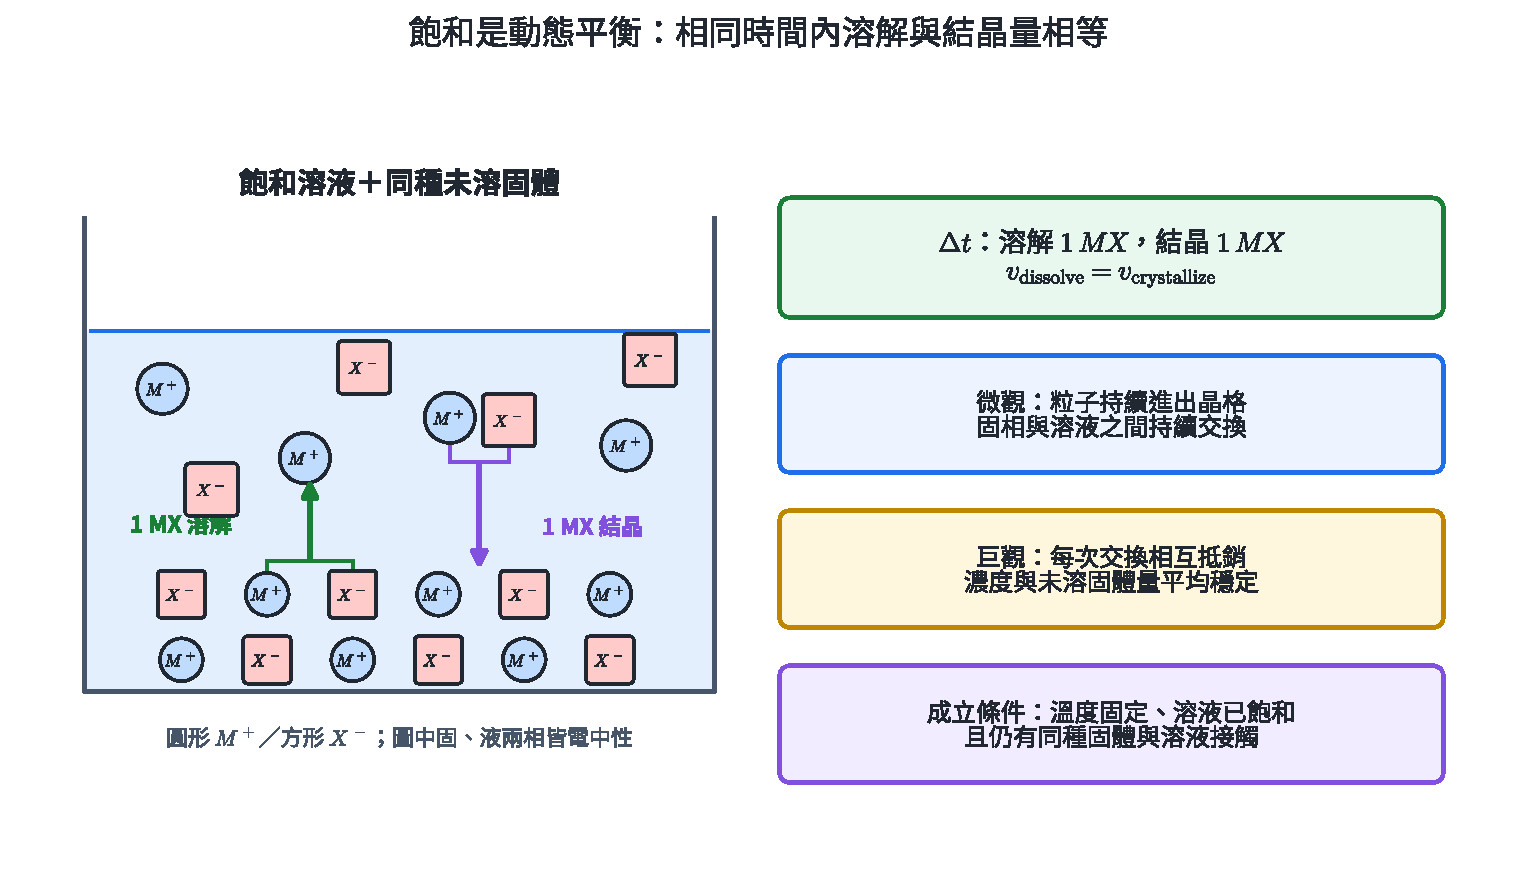
\includegraphics[width=0.96\linewidth,height=\textheight,keepaspectratio,alt={圖 3｜每一段 \textbackslash Delta t 各有一個 MX 溶解與結晶；固、液兩相的離子持續交換，粒子數與電荷保持平衡。}]{assets/必化-3-飽和溶液動態平衡.pdf}
\caption{圖 3｜每一段 \(\Delta t\) 各有一個 \(MX\) 溶解與結晶；固、液兩相的離子持續交換，粒子數與電荷保持平衡。}
\end{figure}

\subsection{2.2 溶解度必須附帶溫度與表示基準}\label{ux6eb6ux89e3ux5ea6ux5fc5ux9808ux9644ux5e36ux6eabux5ea6ux8207ux8868ux793aux57faux6e96}

\textbf{溶解度}是在指定溫度與壓力下，溶質在定量溶劑中形成飽和溶液時的溶質量。固體水溶液常用

\[
S=\frac{m_{\mathrm{solute}}}{m_{\mathrm{water}}}\times100
\]

表示，單位為「\(\mathrm g\) 溶質／\(100\ \mathrm g\) 水」。這個數值的分母是水，不是溶液。

若某物質在 \(25\ ^\circ\mathrm C\) 的溶解度為 \(40\ \mathrm{g}/100\ \mathrm g\) 水，則 \(100\ \mathrm g\) 水最多溶解 \(40\ \mathrm g\) 溶質，形成 \(140\ \mathrm g\) 飽和溶液。其質量百分率為

\[
\frac{40}{100+40}\times100\%=28.6\%.
\]

同一物質也可用莫耳濃度表示飽和濃度，但兩種表示法之間需要莫耳質量與溶液密度才能換算。

\subsection{2.3 溶解度曲線把溫度連到析晶量}\label{ux6eb6ux89e3ux5ea6ux66f2ux7ddaux628aux6eabux5ea6ux9023ux5230ux6790ux6676ux91cf}

多數固體在水中的溶解度隨溫度升高而增加，仍有變化不大或隨溫度下降的例外。溶解度曲線只描述圖中那一種物質與指定溶劑，判讀時不能把「大多數」當成每條曲線都必然上升。

在溶解度---溫度圖上，曲線上的點代表飽和組成；曲線下方代表未達上限；高於曲線的均勻溶液為過飽和狀態。冷卻結晶的計算要固定同一份溶劑質量，分別求高、低溫可留在溶液中的溶質量，再相減。

\begin{figure}
\centering
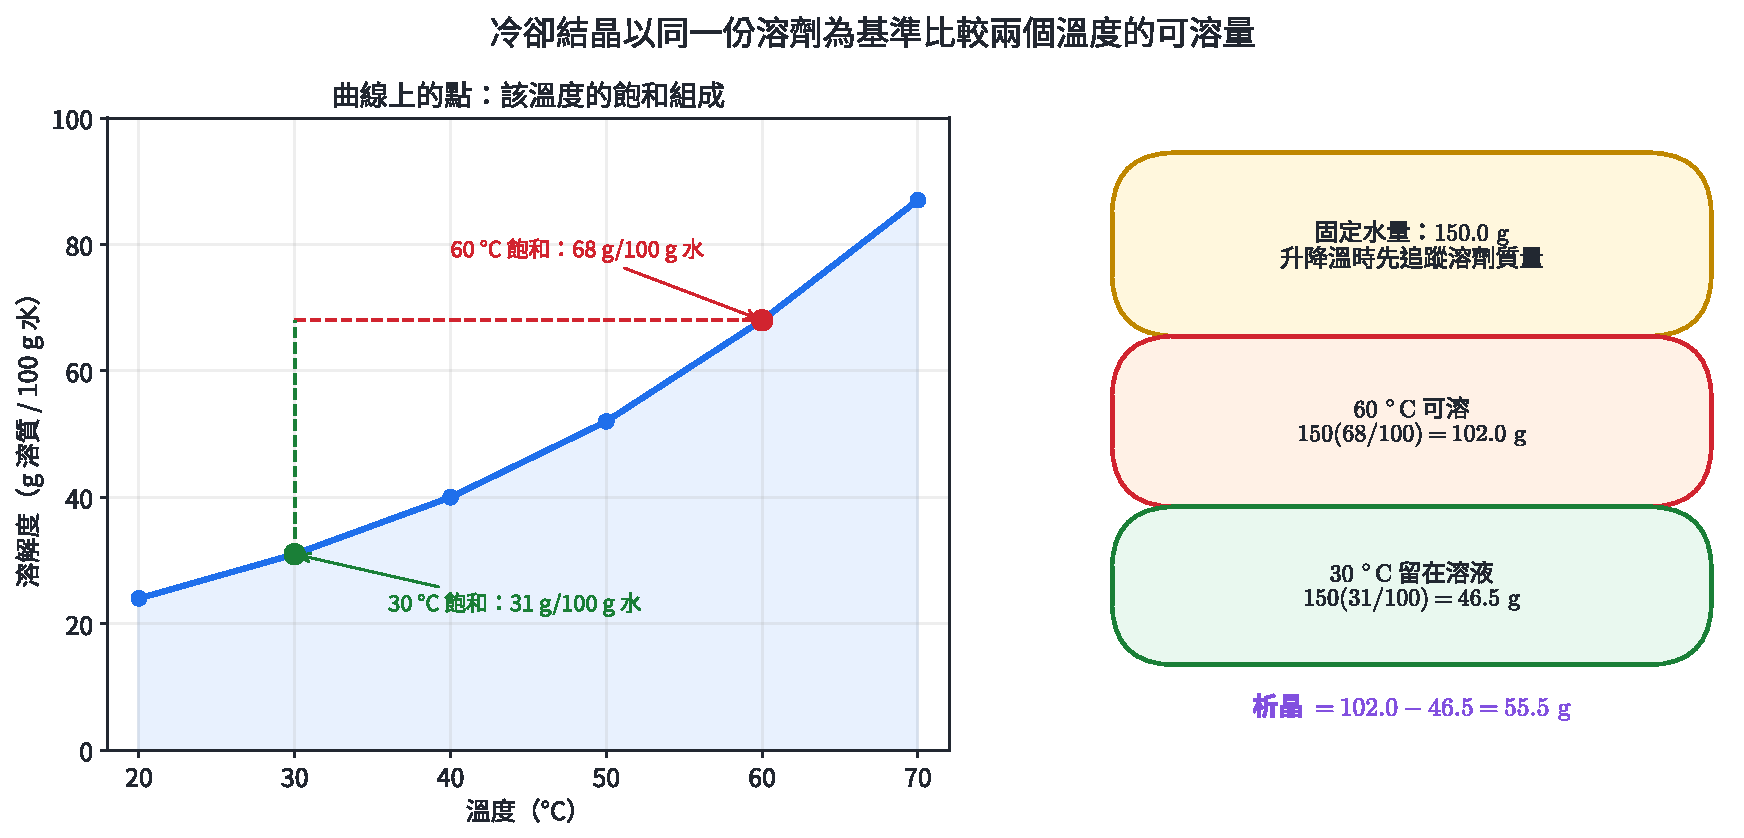
\includegraphics[width=0.98\linewidth,height=\textheight,keepaspectratio,alt={圖 4｜固定 150.0\textbackslash{} \textbackslash mathrm g 水時，由 60\textbackslash{} \^{}\textbackslash circ\textbackslash mathrm C 冷卻到 30\textbackslash{} \^{}\textbackslash circ\textbackslash mathrm C 的可溶量差就是析晶量。}]{assets/必化-3-溶解度曲線與結晶.pdf}
\caption{圖 4｜固定 \(150.0\ \mathrm g\) 水時，由 \(60\ ^\circ\mathrm C\) 冷卻到 \(30\ ^\circ\mathrm C\) 的可溶量差就是析晶量。}
\end{figure}

若冷卻前另有水蒸發，需先扣除蒸發的水，再用低溫溶解度求可留在溶液中的質量。\textbf{溶解度}是比例上限；\textbf{溶解速率}是到達狀態的快慢。攪拌與磨細通常加快溶解，並不改變固定溫度下的平衡溶解度。

\subsection{2.4 氣體溶解度與溫度}\label{ux6c23ux9ad4ux6eb6ux89e3ux5ea6ux8207ux6eabux5ea6}

定壓下，多數氣體在水中的溶解度隨溫度升高而降低。汽水升溫後較容易冒泡，暖水中的溶氧量也通常低於冷水。密閉碳酸飲料同時涉及壓力；本章只使用題目提供的定壓資料，不展開壓力與氣體溶解度的定量定律。

結晶可用於純化固體：選擇溫度敏感度較大的溶解度，讓目標物在高溫溶解、冷卻後結晶，而部分雜質留在母液。所得晶體純度與產率需分別評估；追求大量析晶可能讓雜質一同夾帶。

\textbf{過飽和醋酸鈉的觀察---推論：}透明溶液加入晶種後迅速長出晶體並放熱。直接觀察是晶體前緣擴展與溫度上升；由模型推論，晶種提供成核表面，溶液由過飽和狀態走向飽和平衡。示範涉及加熱玻璃器材與熱溶液，需戴護目鏡與實驗衣、使用耐熱器材並避免封閉加熱；冷卻後的醋酸鈉溶液依教師指定容器回收，不直接倒回試藥瓶。

\begin{HandoutWorkedExample}

\subsection{示範 7｜由溶解度求飽和溶液濃度}\label{ux793aux7bc4-7ux7531ux6eb6ux89e3ux5ea6ux6c42ux98fdux548cux6eb6ux6db2ux6fc3ux5ea6}

\(25\ ^\circ\mathrm C\) 時，溶質 X 的溶解度為 \(45.0\ \mathrm g/100\ \mathrm g\) 水。求飽和溶液的質量百分率。

以 \(100.0\ \mathrm g\) 水為基準，飽和時含 \(45.0\ \mathrm g\) X，溶液總質量為 \(145.0\ \mathrm g\)：

\[
w\%=\frac{45.0}{145.0}\times100\%=31.0\%.
\]

\end{HandoutWorkedExample}

\begin{HandoutWorkedExample}

\subsection{示範 8｜判斷不飽和、飽和與剩餘固體}\label{ux793aux7bc4-8ux5224ux65b7ux4e0dux98fdux548cux98fdux548cux8207ux5269ux9918ux56faux9ad4}

\(40\ ^\circ\mathrm C\) 時，X 的溶解度為 \(40.0\ \mathrm g/100\ \mathrm g\) 水。分別將 \(30.0\ \mathrm g\) 與 \(50.0\ \mathrm g\) X 加入兩杯各含 \(100.0\ \mathrm g\) 水的燒杯。

第一杯的 \(30.0\ \mathrm g<40.0\ \mathrm g\)，完全溶解後為不飽和溶液。第二杯最多溶解 \(40.0\ \mathrm g\)，形成飽和溶液並剩餘

\[
50.0-40.0=10.0\ \mathrm g
\]

固體。兩杯水量相同，才能直接把加入量與 \(40.0\ \mathrm g/100\ \mathrm g\) 水比較。

\end{HandoutWorkedExample}

\begin{HandoutWorkedExample}

\subsection{示範 9｜由曲線資料求冷卻析晶量}\label{ux793aux7bc4-9ux7531ux66f2ux7ddaux8cc7ux6599ux6c42ux51b7ux537bux6790ux6676ux91cf}

某溶質在 \(60\ ^\circ\mathrm C\) 與 \(30\ ^\circ\mathrm C\) 的溶解度分別為 \(68.0\) 與 \(31.0\ \mathrm g/100\ \mathrm g\) 水。以 \(150.0\ \mathrm g\) 水配成 \(60\ ^\circ\mathrm C\) 飽和溶液，再冷卻至 \(30\ ^\circ\mathrm C\)，求析晶量；忽略水分蒸發。

高溫已溶質量：

\[
m_{60}=150.0\times\frac{68.0}{100}=102.0\ \mathrm g.
\]

低溫仍可溶質量：

\[
m_{30}=150.0\times\frac{31.0}{100}=46.5\ \mathrm g.
\]

\[
m_{\mathrm{crystal}}=102.0-46.5=55.5\ \mathrm g.
\]

\end{HandoutWorkedExample}

\begin{HandoutWorkedExample}

\subsection{示範 10｜蒸發與降溫同時發生}\label{ux793aux7bc4-10ux84b8ux767cux8207ux964dux6eabux540cux6642ux767cux751f}

某物質在 \(80\ ^\circ\mathrm C\) 與 \(20\ ^\circ\mathrm C\) 的溶解度分別為 \(100\) 與 \(25.0\ \mathrm g/100\ \mathrm g\) 水。取 \(300\ \mathrm g\) 的 \(80\ ^\circ\mathrm C\) 飽和溶液，先蒸發 \(30.0\ \mathrm g\) 水，再冷卻至 \(20\ ^\circ\mathrm C\)。求析晶量。

\(80\ ^\circ\mathrm C\) 飽和組成為 \(100\ \mathrm g\) 溶質配 \(100\ \mathrm g\) 水，故 \(300\ \mathrm g\) 溶液含水與溶質各 \(150\ \mathrm g\)。

蒸發後水剩

\[
150-30.0=120\ \mathrm g.
\]

\(20\ ^\circ\mathrm C\) 時可留在溶液中的溶質為

\[
120\times\frac{25.0}{100}=30.0\ \mathrm g.
\]

故析晶量為

\[
150-30.0=120\ \mathrm g.
\]

\end{HandoutWorkedExample}

\begin{HandoutWorkedExample}

\subsection{示範 11｜氣體溶解度資料}\label{ux793aux7bc4-11ux6c23ux9ad4ux6eb6ux89e3ux5ea6ux8cc7ux6599}

定壓下，某氣體在 \(20\ ^\circ\mathrm C\) 與 \(40\ ^\circ\mathrm C\) 的溶解度分別為 \(0.170\) 與 \(0.100\ \mathrm g/100\ \mathrm g\) 水。\(500\ \mathrm g\) 水在 \(20\ ^\circ\mathrm C\) 已達飽和，升至 \(40\ ^\circ\mathrm C\) 並重新達平衡，估計逸出氣體質量。

\[
m_{20}=500\times\frac{0.170}{100}=0.850\ \mathrm g,
\]

\[
m_{40}=500\times\frac{0.100}{100}=0.500\ \mathrm g.
\]

逸出量為

\[
0.850-0.500=0.350\ \mathrm g.
\]

\end{HandoutWorkedExample}

\subsection{練習 2}\label{ux7df4ux7fd2-2}

\begin{enumerate}
\def\labelenumi{\arabic{enumi}.}
\tightlist
\item
  \(30\ ^\circ\mathrm C\) 時，Y 的溶解度為 \(20.0\ \mathrm g/100\ \mathrm g\) 水。\(50.0\ \mathrm g\) 水最多溶解多少 Y？
\item
  上題形成的飽和溶液質量百分率為多少？
\item
  \(70\ ^\circ\mathrm C\) 時，Z 的溶解度為 \(80.0\ \mathrm g/100\ \mathrm g\) 水；\(20\ ^\circ\mathrm C\) 時為 \(30.0\ \mathrm g/100\ \mathrm g\) 水。以 \(200\ \mathrm g\) 水配成高溫飽和溶液後冷卻，求析晶量。
\item
  某杯在 \(25\ ^\circ\mathrm C\) 含 \(100\ \mathrm g\) 水與 \(35\ \mathrm g\) 溶質，該溫度溶解度為 \(40\ \mathrm g/100\ \mathrm g\) 水。判斷狀態，並求再加多少溶質可達飽和。
\item
  固體研磨、攪拌與升溫三種操作中，哪些通常提高溶解速率？哪些可能改變固體平衡溶解度？
\item
  定壓下，氣體 Q 在 \(10\ ^\circ\mathrm C\) 與 \(30\ ^\circ\mathrm C\) 的溶解度為 \(0.240\) 與 \(0.150\ \mathrm g/100\ \mathrm g\) 水。\(800\ \mathrm g\) 飽和水溶液由 \(10\ ^\circ\mathrm C\) 升至 \(30\ ^\circ\mathrm C\)，估計逸出質量。
\end{enumerate}

\subsection{練習 2 解析}\label{ux7df4ux7fd2-2-ux89e3ux6790}

\begin{enumerate}
\def\labelenumi{\arabic{enumi}.}
\tightlist
\item
  \(50.0(20.0/100)=10.0\ \mathrm g\)。
\item
  飽和溶液質量為 \(50.0+10.0=60.0\ \mathrm g\)，故 \(10.0/60.0\times100\%=16.7\%\)。
\item
  高溫可溶 \(200(80.0/100)=160\ \mathrm g\)，低溫可留 \(200(30.0/100)=60.0\ \mathrm g\)，析晶 \(100\ \mathrm g\)。
\item
  \(35<40\)，是不飽和溶液；再加 \(5.0\ \mathrm g\) 可達飽和。
\item
  研磨與攪拌增加接觸或傳質，通常提高速率；升溫通常提高速率，也可能改變平衡溶解度。研磨與攪拌在固定溫度下不改變溶解度。
\item
  逸出量為 \(800(0.240-0.150)/100=0.720\ \mathrm g\)。
\end{enumerate}

\section{3. 酸鹼、水的離子積、pH 與中和}\label{ux9178ux9e7cux6c34ux7684ux96e2ux5b50ux7a4dph-ux8207ux4e2dux548c}

\subsection{3.1 阿瑞尼斯酸鹼以水溶液中的離子定義}\label{ux963fux745eux5c3cux65afux9178ux9e7cux4ee5ux6c34ux6eb6ux6db2ux4e2dux7684ux96e2ux5b50ux5b9aux7fa9}

依阿瑞尼斯模型，\textbf{酸}是在水中使 \(H^+\) 濃度增加的物質，\textbf{鹼}是在水中使 \(OH^-\) 濃度增加的物質。水溶液中的裸露質子實際與水分子作用，常寫成 \(H_3O^+\)；高中計算以 \(H^+\) 簡寫。

\[
HCl(aq)\rightarrow H^+(aq)+Cl^-(aq),
\]

\[
NaOH(aq)\rightarrow Na^+(aq)+OH^-(aq).
\]

\textbf{強酸、強鹼}在一般稀水溶液中近乎完全游離；\textbf{弱酸、弱鹼}只有一部分粒子形成離子。例如

\[
CH_3COOH(aq)\rightleftharpoons H^+(aq)+CH_3COO^-(aq).
\]

強弱描述游離程度，濃淡描述每單位體積的物質量。稀的強酸可以有較低 \([H^+]\)，濃的弱酸也可能有較高 \([H^+]\)；判斷時需同時知道種類與濃度。

\begin{figure}
\centering
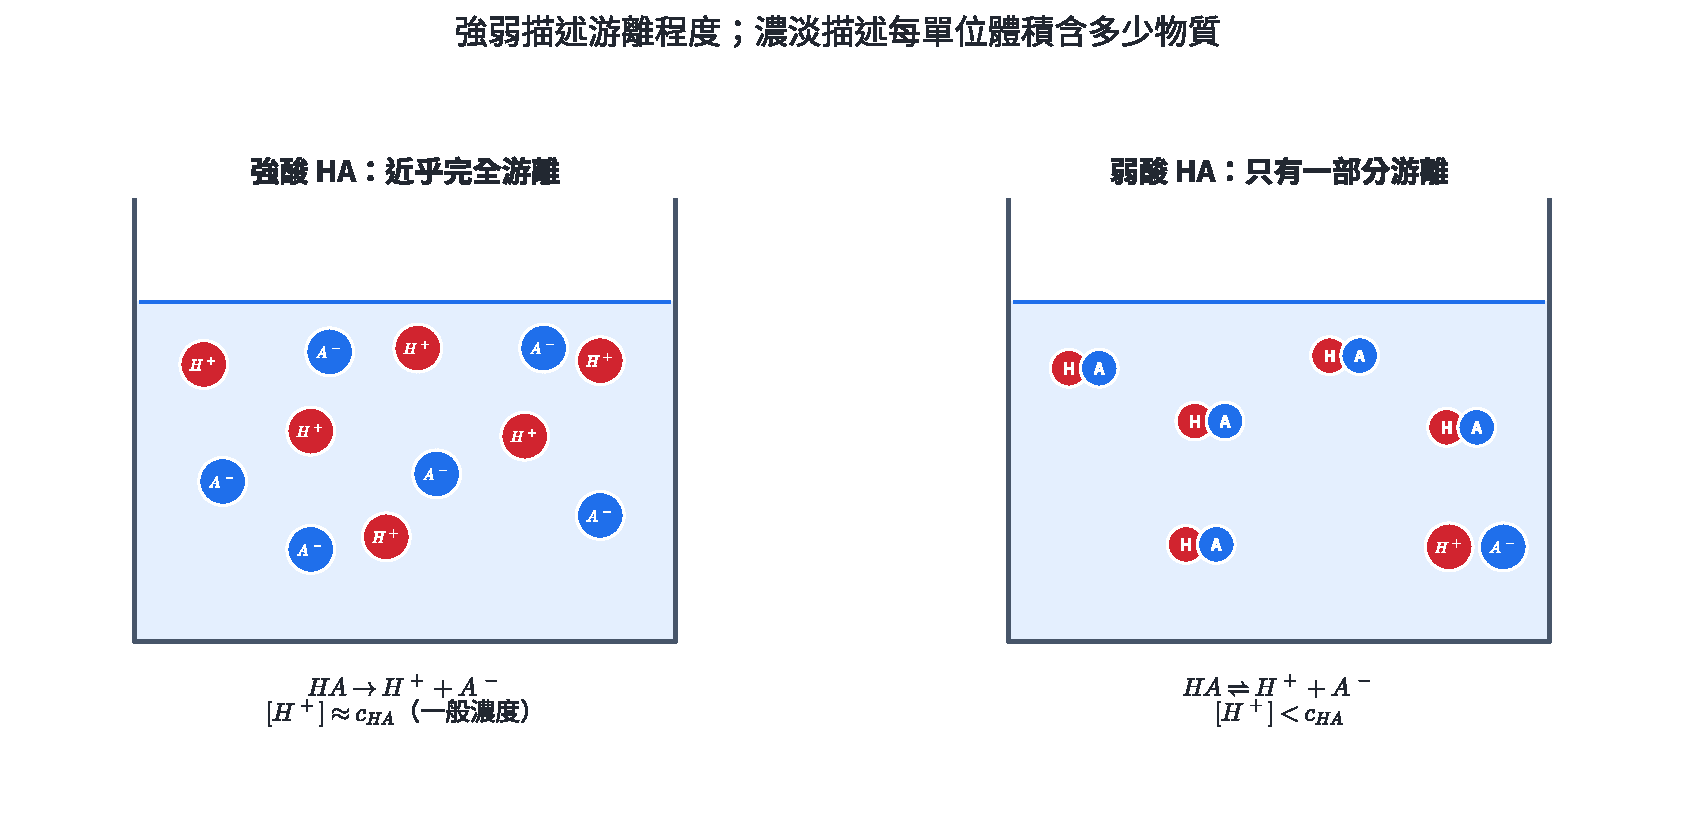
\includegraphics[width=0.96\linewidth,height=\textheight,keepaspectratio,alt={圖 5｜相同分析濃度下，強酸近乎全部成為離子，弱酸多數仍以未游離分子存在。}]{assets/必化-3-強弱酸鹼粒子模型.pdf}
\caption{圖 5｜相同分析濃度下，強酸近乎全部成為離子，弱酸多數仍以未游離分子存在。}
\end{figure}

酸性水溶液可使藍色石蕊變紅，常與活性足夠的金屬產生氫氣，亦可與碳酸鹽產生二氧化碳；鹼性水溶液可使紅色石蕊變藍，並可與油脂發生反應。氣味、腐蝕性與濃度會改變感官，實驗室以指示劑、pH 計或反應證據測試，禁止以口嚐或皮膚觸摸辨認酸鹼。

\subsection{\texorpdfstring{3.2 水的離子積連接 \(H^+\) 與 \(OH^-\)}{3.2 水的離子積連接 H\^{}+ 與 OH\^{}-}}\label{ux6c34ux7684ux96e2ux5b50ux7a4dux9023ux63a5-h-ux8207-oh-}

水會微量自解離：

\[
H_2O(l)\rightleftharpoons H^+(aq)+OH^-(aq).
\]

固定溫度下，水溶液滿足

\[
K_w=[H^+][OH^-].
\]

在 \(25\ ^\circ\mathrm C\)，

\[
K_w=1.0\times10^{-14}.
\]

加入酸或鹼會改變 \([H^+]\) 與 \([OH^-]\)，同溫下兩者乘積仍為 \(K_w\)。\(K_w\) 隨溫度改變；\textbf{中性}的定義始終是 \([H^+]=[OH^-]\)，只有在 \(25\ ^\circ\mathrm C\) 時中性 pH 為 7.00。

\subsection{3.3 pH 把跨越多個數量級的濃度壓縮成對數}\label{ph-ux628aux8de8ux8d8aux591aux500bux6578ux91cfux7d1aux7684ux6fc3ux5ea6ux58d3ux7e2eux6210ux5c0dux6578}

\[
pH=-\log[H^+],\qquad pOH=-\log[OH^-],
\]

\[
pK_w=-\log K_w=pH+pOH.
\]

在 \(25\ ^\circ\mathrm C\)，\(pK_w=14.00\)。pH 每增加 1，\([H^+]\) 變為原來的 \(1/10\)；pH 相差 3 表示 \([H^+]\) 相差 \(10^3\) 倍。pH 是對數量，不能直接把兩杯溶液的 pH 做算術平均來求混合結果。

\begin{figure}
\centering
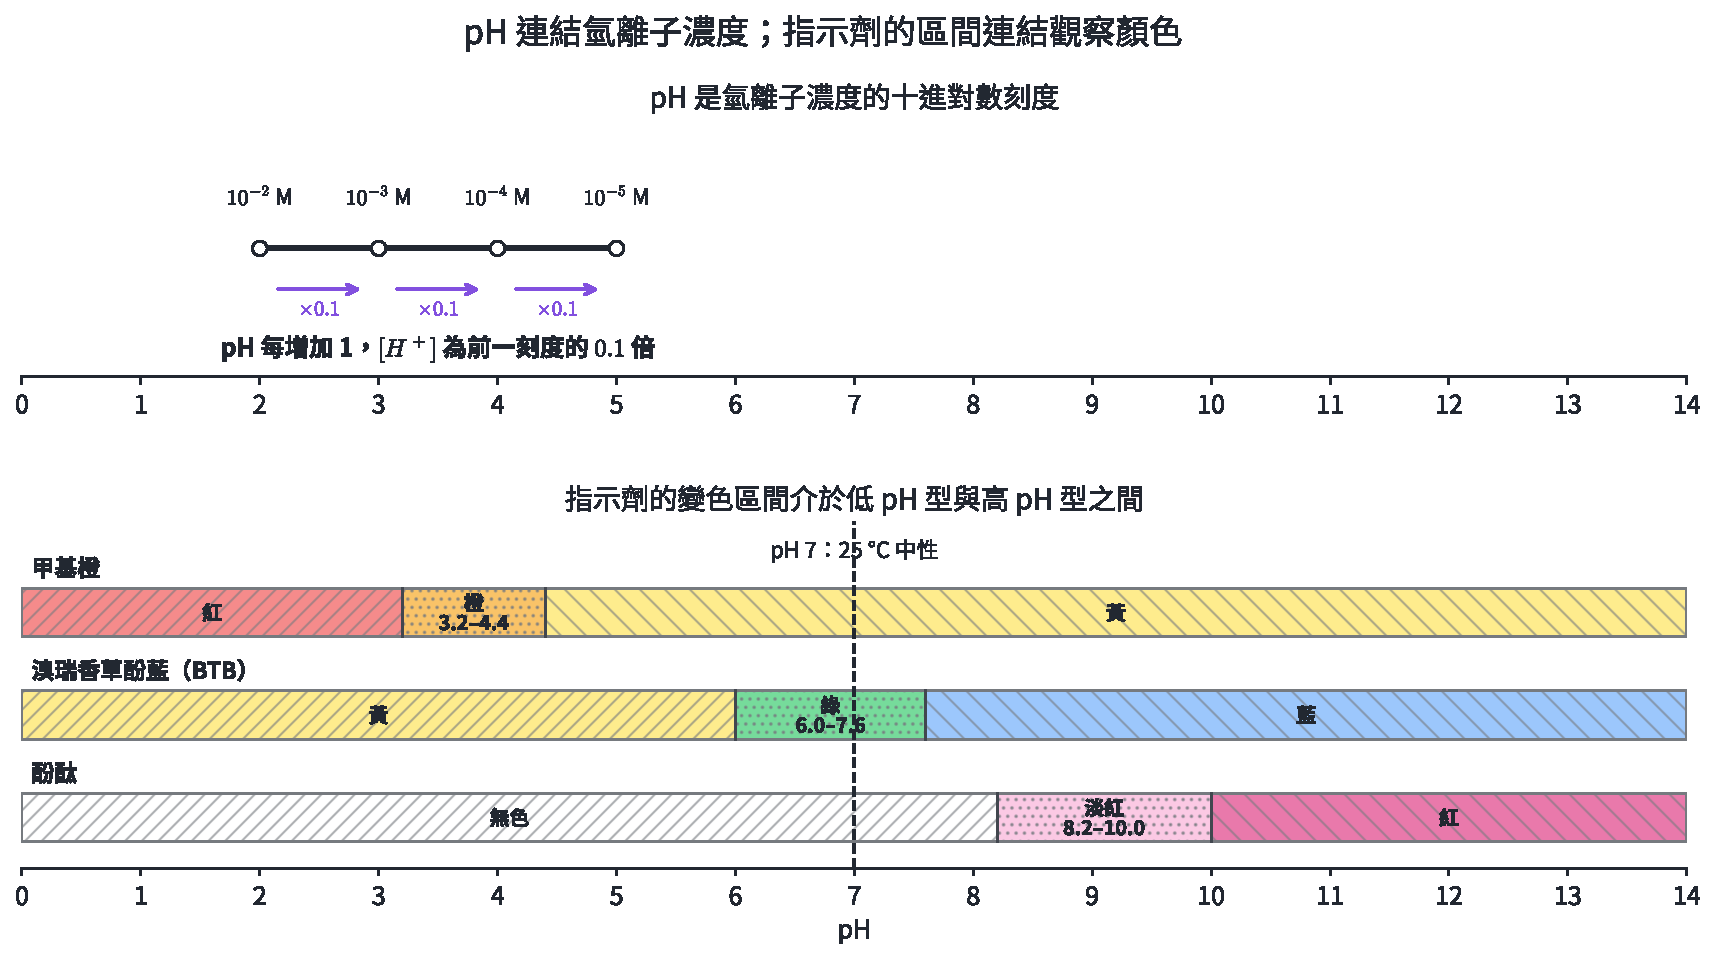
\includegraphics[width=0.98\linewidth,height=\textheight,keepaspectratio,alt={圖 6｜pH 每增加 1，H\^{}+ 濃度為前一刻度的 0.1 倍；每列以區段文字與紋理標出指示劑的低 pH 型、變色區與高 pH 型。}]{assets/必化-3-pH與指示劑範圍.pdf}
\caption{圖 6｜pH 每增加 1，\(H^+\) 濃度為前一刻度的 \(0.1\) 倍；每列以區段文字與紋理標出指示劑的低 pH 型、變色區與高 pH 型。}
\end{figure}

本章的強酸、強鹼 pH 計算使用題目指定的一般濃度，令完全游離所給出的 \([H^+]\) 或 \([OH^-]\) 遠大於純水的 \(10^{-7}\ \mathrm M\)。當分析濃度接近或低於 \(10^{-7}\ \mathrm M\)，水自解離不可忽略，需使用後續平衡模型。

\subsection{3.4 指示劑以變色範圍提供區間證據}\label{ux6307ux793aux5291ux4ee5ux8b8aux8272ux7bc4ux570dux63d0ux4f9bux5340ux9593ux8b49ux64da}

酸鹼指示劑通常是弱酸或弱鹼，其兩種型態顏色不同。每種指示劑在特定 pH 範圍逐漸變色，例如：

{\def\LTcaptype{none} % do not increment counter
\begin{longtable}[]{@{}lrrr@{}}
\toprule\noalign{}
指示劑 & 低 pH 顏色 & 變色範圍 & 高 pH 顏色 \\
\midrule\noalign{}
\endhead
\bottomrule\noalign{}
\endlastfoot
甲基橙 & 紅 & 3.2--4.4 & 黃 \\
溴瑞香草酚藍（BTB） & 黃 & 6.0--7.6 & 藍 \\
酚酞 & 無色 & 8.2--10.0 & 粉紅 \\
\end{longtable}
}

若某溶液使甲基橙呈黃、BTB 呈黃、酚酞無色，資料共同支持 \(4.4<pH<6.0\)。指示劑只能給範圍；pH 計經校正後可提供數值。

紫甘藍色素可作為多色指示劑。微量測試仍需護目鏡與實驗衣；酸、鹼溶液依標示濃度使用滴管，避免交叉污染。若使用含乙醇的商用指示劑，需遠離火源。觀察記錄寫「顏色由紫轉紅／綠」；「溶液偏酸／偏鹼」是依色卡與對照組得到的推論。廢液依酸鹼與有機溶劑分類處理。

\subsection{3.5 中和先做反應計量，再判斷剩餘粒子}\label{ux4e2dux548cux5148ux505aux53cdux61c9ux8a08ux91cfux518dux5224ux65b7ux5269ux9918ux7c92ux5b50}

酸與鹼反應生成鹽與水。強酸、強鹼的核心淨離子反應為

\[
H^+(aq)+OH^-(aq)\rightarrow H_2O(l).
\]

計算依序是：把各溶液換成 \(H^+\)、\(OH^-\) 莫耳數；依 \(1:1\) 反應；找出剩餘者；除以混合後總體積；最後求 pH。多質子酸或多羥基鹼要由化學式與反應式計入每莫耳可提供的 \(H^+\) 或 \(OH^-\)。

\begin{figure}
\centering
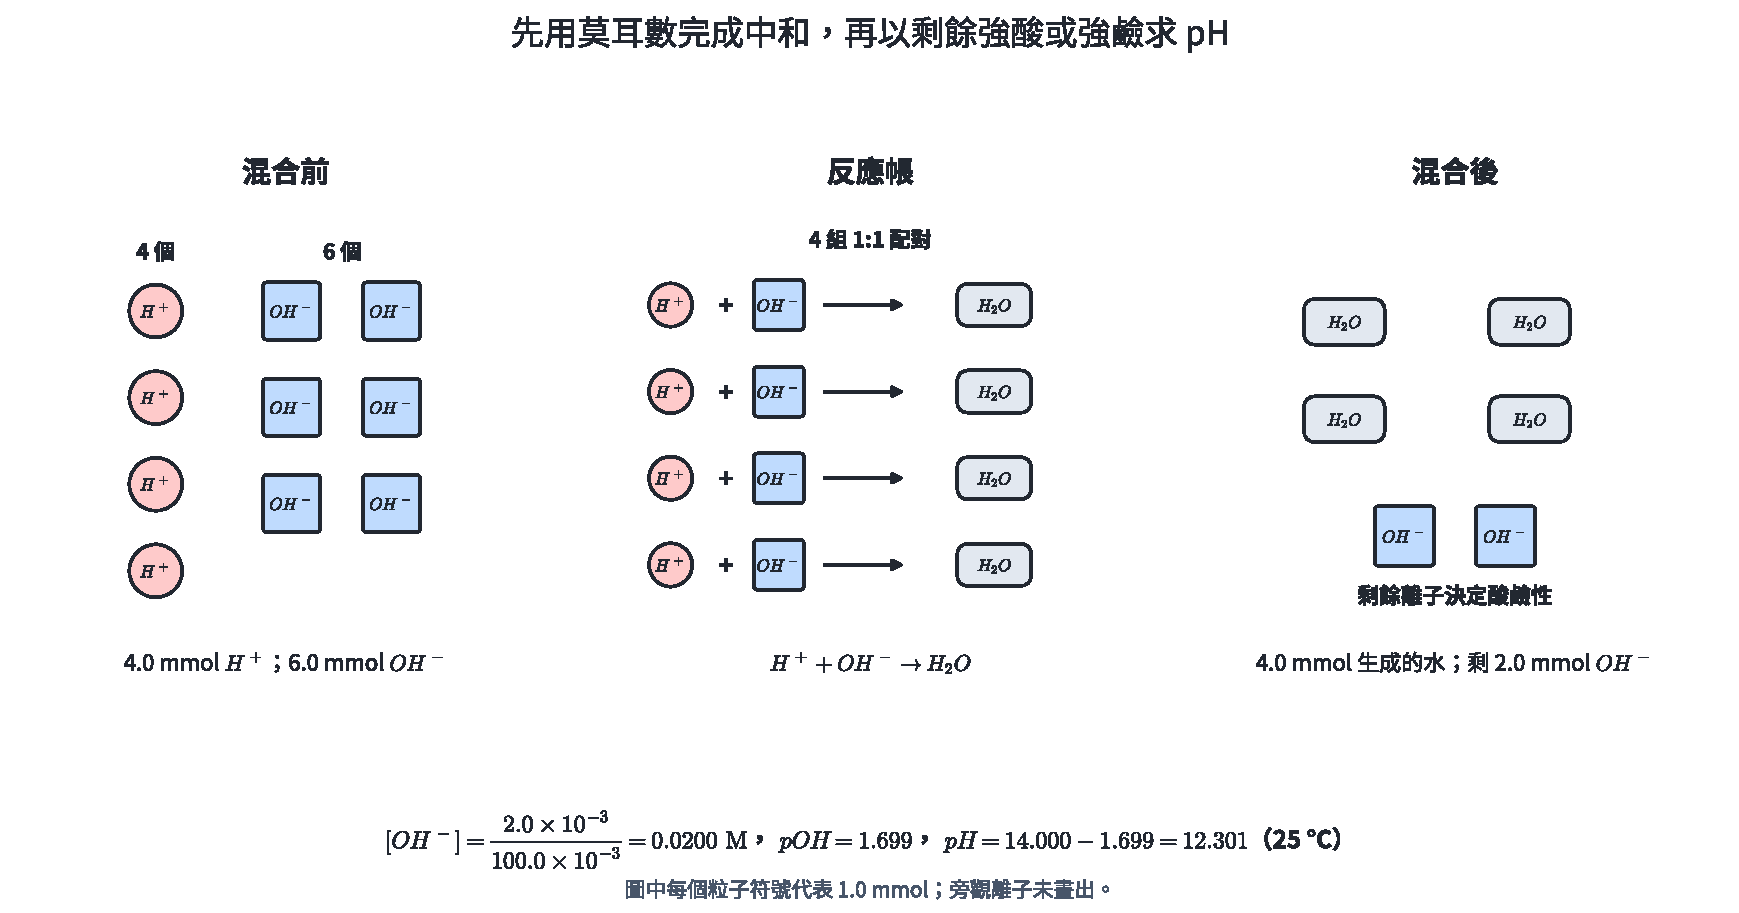
\includegraphics[width=0.98\linewidth,height=\textheight,keepaspectratio,alt={圖 7｜每個粒子符號代表 1.0\textbackslash{} \textbackslash mathrm\{mmol\}；4 個 H\^{}+ 消耗 6 個 OH\^{}- 中的 4 個，生成 4.0\textbackslash{} \textbackslash mathrm\{mmol\} 水並留下 2.0\textbackslash{} \textbackslash mathrm\{mmol\} OH\^{}-。}]{assets/必化-3-中和反應粒子帳.pdf}
\caption{圖 7｜每個粒子符號代表 \(1.0\ \mathrm{mmol}\)；4 個 \(H^+\) 消耗 6 個 \(OH^-\) 中的 4 個，生成 \(4.0\ \mathrm{mmol}\) 水並留下 \(2.0\ \mathrm{mmol}\) \(OH^-\)。}
\end{figure}

中和反應通常放熱。滴定或混合實驗需戴護目鏡與實驗衣，使用適當濃度與小體積；強酸強鹼具有腐蝕性，盛裝與廢液處理依實驗室規範。中和後的 pH 仍由反應物強弱、比例與鹽類性質決定，不能只因「發生中和」就預設為 7。

酸鹼計量可直接用於制酸劑有效成分、廢水中和與食品製程酸度控制。藥品使用仍依標示與專業建議；化學式計算只回答理論中和量。

\begin{HandoutWorkedExample}

\subsection{示範 12｜由強酸濃度求 pH}\label{ux793aux7bc4-12ux7531ux5f37ux9178ux6fc3ux5ea6ux6c42-ph}

\(25\ ^\circ\mathrm C\) 時，\(3.0\times10^{-4}\ \mathrm M\) HCl 的 pH、pOH 與 \([OH^-]\) 為何？

HCl 近乎完全游離：

\[
[H^+]=3.0\times10^{-4}\ \mathrm M.
\]

\[
pH=-\log(3.0\times10^{-4})=4-\log3.0=3.52.
\]

\[
pOH=14.00-3.52=10.48,
\]

\[
[OH^-]=\frac{1.0\times10^{-14}}{3.0\times10^{-4}}
=3.3\times10^{-11}\ \mathrm M.
\]

\end{HandoutWorkedExample}

\begin{HandoutWorkedExample}

\subsection{示範 13｜由強鹼濃度求 pH}\label{ux793aux7bc4-13ux7531ux5f37ux9e7cux6fc3ux5ea6ux6c42-ph}

\(25\ ^\circ\mathrm C\) 時，\(0.0200\ \mathrm M\) NaOH 的 pH 為何？

\[
[OH^-]=0.0200=2.00\times10^{-2}\ \mathrm M,
\]

\[
pOH=-\log(2.00\times10^{-2})=1.699,
\]

\[
pH=14.000-1.699=12.301.
\]

\end{HandoutWorkedExample}

\begin{HandoutWorkedExample}

\subsection{示範 14｜稀釋後的強酸 pH}\label{ux793aux7bc4-14ux7a00ux91cbux5f8cux7684ux5f37ux9178-ph}

取 \(2.00\ \mathrm{mL}\)、\(0.100\ \mathrm M\) HCl，加水至 \(250.0\ \mathrm{mL}\)。求 \(25\ ^\circ\mathrm C\) 的 pH。

稀釋保存 HCl 莫耳數：

\[
C_2=\frac{(0.100)(2.00)}{250.0}=8.00\times10^{-4}\ \mathrm M.
\]

\[
pH=-\log(8.00\times10^{-4})=3.097.
\]

此濃度遠大於 \(10^{-7}\ \mathrm M\)，可用完全游離的強酸近似。

\end{HandoutWorkedExample}

\begin{HandoutWorkedExample}

\subsection{示範 15｜由指示劑交集限制 pH}\label{ux793aux7bc4-15ux7531ux6307ux793aux5291ux4ea4ux96c6ux9650ux5236-ph}

某無色水溶液使甲基橙呈黃、BTB 呈綠、酚酞無色。依表中範圍判斷 pH 區間。

甲基橙呈黃支持 \(pH>4.4\)；BTB 呈綠表示落在其變色區，\(6.0<pH<7.6\)；酚酞無色支持 \(pH<8.2\)。三項交集仍是

\[
6.0<pH<7.6.
\]

顏色受觀察與濃度影響，答案是區間而非單一 pH。

\end{HandoutWorkedExample}

\begin{HandoutWorkedExample}

\subsection{示範 16｜強酸強鹼混合後的 pH}\label{ux793aux7bc4-16ux5f37ux9178ux5f37ux9e7cux6df7ux5408ux5f8cux7684-ph}

將 \(25.0\ \mathrm{mL}\)、\(0.120\ \mathrm M\) \(H_2SO_4\) 與 \(40.0\ \mathrm{mL}\)、\(0.100\ \mathrm M\) NaOH 混合。依高中常用模型把兩個酸性氫都視為可完全中和，求 \(25\ ^\circ\mathrm C\) 的 pH。

酸所提供的 \(H^+\)：

\[
n(H^+)=2(0.120)(0.0250)=0.00600\ \mathrm{mol}.
\]

鹼所提供的 \(OH^-\)：

\[
n(OH^-)=(0.100)(0.0400)=0.00400\ \mathrm{mol}.
\]

反應後剩 \(0.00200\ \mathrm{mol}\) \(H^+\)，總體積為 \(0.0650\ \mathrm L\)：

\[
[H^+]=\frac{0.00200}{0.0650}=0.0308\ \mathrm M,
\]

\[
pH=-\log(0.0308)=1.51.
\]

\end{HandoutWorkedExample}

\begin{HandoutWorkedExample}

\subsection{示範 17｜制酸劑的理論中和量}\label{ux793aux7bc4-17ux5236ux9178ux5291ux7684ux7406ux8ad6ux4e2dux548cux91cf}

一錠制酸劑含 \(0.200\ \mathrm g\) \(Mg(OH)_2\)。取 \(M=58.3\ \mathrm{g\,mol^{-1}}\)，求可中和多少毫升 \(0.100\ \mathrm M\) HCl。

\[
n\bigl(Mg(OH)_2\bigr)=\frac{0.200}{58.3}=3.43\times10^{-3}\ \mathrm{mol}.
\]

由

\[
Mg(OH)_2+2HCl\rightarrow MgCl_2+2H_2O,
\]

可中和

\[
n(HCl)=2(3.43\times10^{-3})=6.86\times10^{-3}\ \mathrm{mol}.
\]

\[
V=\frac{n}{C}=\frac{6.86\times10^{-3}}{0.100}
=0.0686\ \mathrm L=68.6\ \mathrm{mL}.
\]

\end{HandoutWorkedExample}

\subsection{練習 3}\label{ux7df4ux7fd2-3}

\begin{enumerate}
\def\labelenumi{\arabic{enumi}.}
\tightlist
\item
  \(25\ ^\circ\mathrm C\) 時，\([H^+]=2.0\times10^{-5}\ \mathrm M\)，求 pH、pOH 與 \([OH^-]\)。
\item
  \(25\ ^\circ\mathrm C\) 時，\([OH^-]=5.0\times10^{-3}\ \mathrm M\)，求 pH。
\item
  pH 3.0 與 pH 6.0 的兩溶液，前者 \([H^+]\) 是後者幾倍？
\item
  取 \(10.0\ \mathrm{mL}\)、\(0.500\ \mathrm M\) HCl 加水至 \(250.0\ \mathrm{mL}\)，求 pH。
\item
  混合 \(30.0\ \mathrm{mL}\)、\(0.100\ \mathrm M\) HCl 與 \(20.0\ \mathrm{mL}\)、\(0.100\ \mathrm M\) NaOH，求 \(25\ ^\circ\mathrm C\) 的 pH。
\item
  某溶液使甲基橙呈黃、BTB 呈藍、酚酞呈無色。依表中範圍寫出最窄 pH 區間。
\end{enumerate}

\subsection{練習 3 解析}\label{ux7df4ux7fd2-3-ux89e3ux6790}

\begin{enumerate}
\def\labelenumi{\arabic{enumi}.}
\tightlist
\item
  \(pH=4.70\)；\(pOH=9.30\)；\([OH^-]=1.0\times10^{-14}/(2.0\times10^{-5})=5.0\times10^{-10}\ \mathrm M\)。
\item
  \(pOH=-\log(5.0\times10^{-3})=2.30\)，故 \(pH=11.70\)。
\item
  \(10^{-3}/10^{-6}=10^3\)，是 \(1000\) 倍。
\item
  稀釋後 \([H^+]=(0.500)(10.0)/250.0=0.0200\ \mathrm M\)，故 \(pH=1.70\)。
\item
  \(H^+\) 為 \(3.00\ \mathrm{mmol}\)，\(OH^-\) 為 \(2.00\ \mathrm{mmol}\)，剩 \(1.00\ \mathrm{mmol}\) 於 \(50.0\ \mathrm{mL}\)；\([H^+]=0.0200\ \mathrm M\)，\(pH=1.70\)。
\item
  甲基橙黃：\(pH>4.4\)；BTB 藍：\(pH>7.6\)；酚酞無色：\(pH<8.2\)。交集為 \(7.6<pH<8.2\)。
\end{enumerate}

\section{4. 氧化還原、氧化劑與還原劑}\label{ux6c27ux5316ux9084ux539fux6c27ux5316ux5291ux8207ux9084ux539fux5291}

\subsection{4.1 氧的轉移是特例，電子轉移是共同模型}\label{ux6c27ux7684ux8f49ux79fbux662fux7279ux4f8bux96fbux5b50ux8f49ux79fbux662fux5171ux540cux6a21ux578b}

以氧的轉移描述時，物質\textbf{得到氧}稱為氧化，氧化物\textbf{失去氧}稱為還原。例如

\[
CuO(s)+H_2(g)\rightarrow Cu(s)+H_2O(g)
\]

中，\(H_2\) 得到氧形成水，\(H_2\) 被氧化；\(CuO\) 失去氧形成 Cu，\(CuO\) 被還原。

更廣義的定義是：

\begin{itemize}
\tightlist
\item
  \textbf{氧化：}粒子失去電子。
\item
  \textbf{還原：}粒子得到電子。
\end{itemize}

電子由一方轉移到另一方，故氧化與還原同時發生，失去與得到的電子數相等。反應不一定含氧，例如

\[
Fe(s)+Cu^{2+}(aq)\rightarrow Fe^{2+}(aq)+Cu(s).
\]

其中

\[
Fe(s)\rightarrow Fe^{2+}(aq)+2e^-,
\]

\[
Cu^{2+}(aq)+2e^-\rightarrow Cu(s).
\]

\begin{figure}
\centering
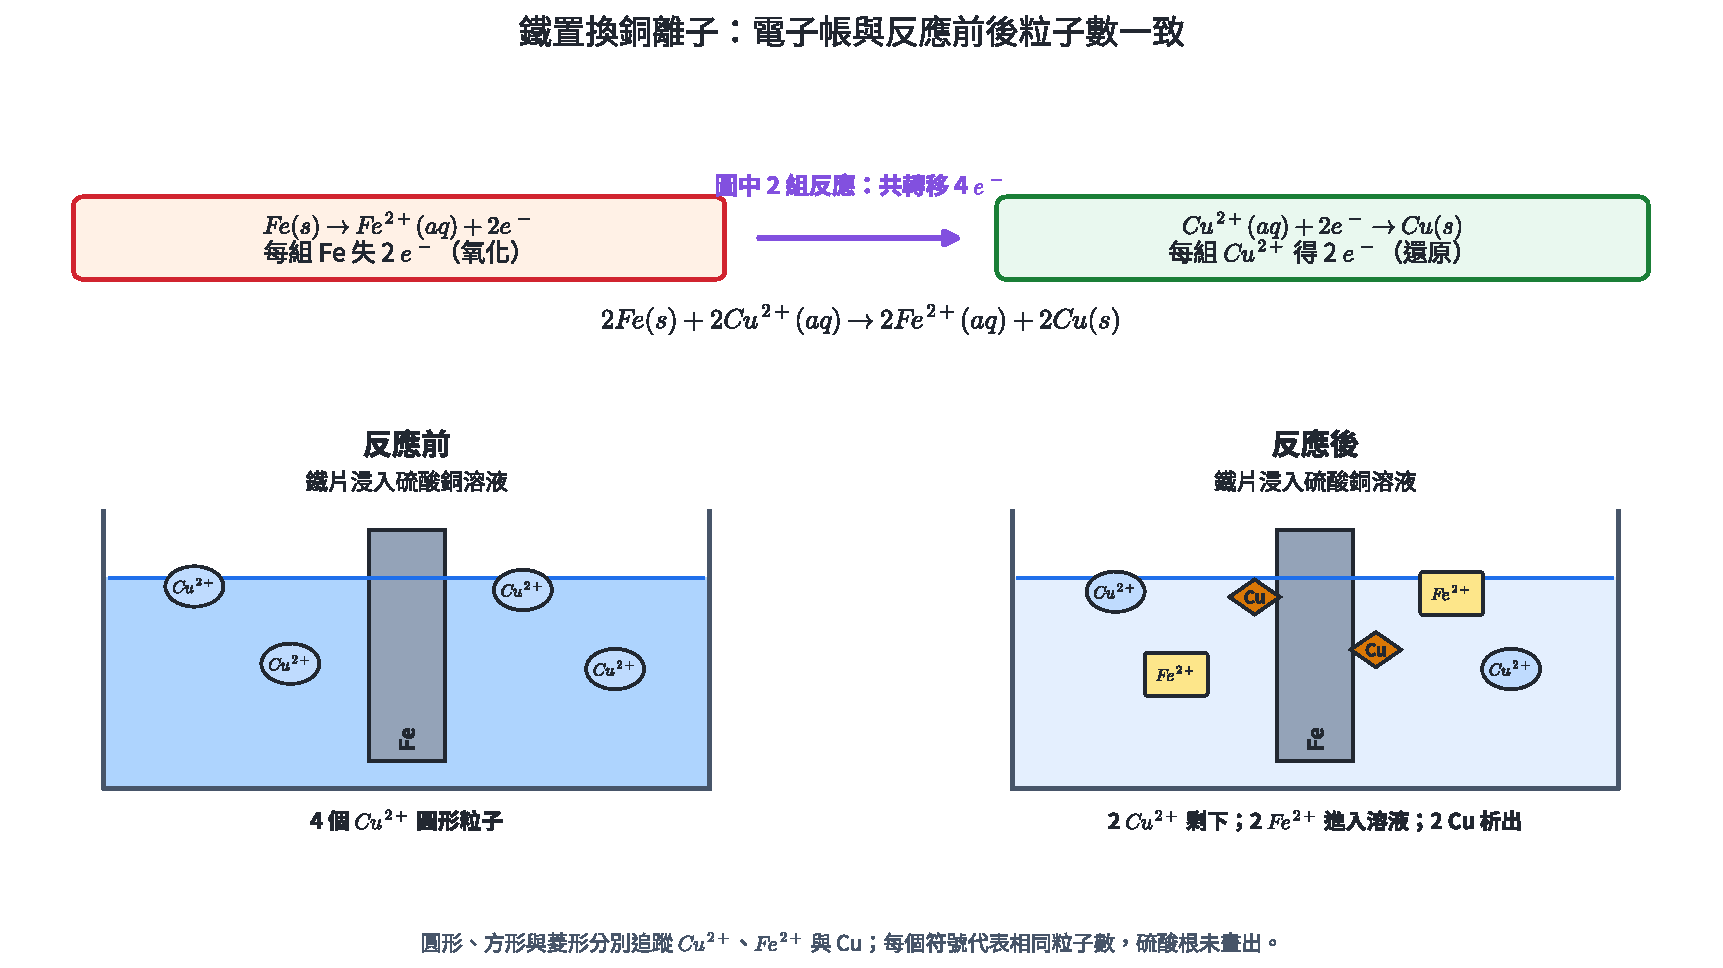
\includegraphics[width=0.98\linewidth,height=\textheight,keepaspectratio,alt={圖 8｜圖中 2 組等量反應消耗 2 個 Cu\^{}\{2+\}，生成 2 個 Fe\^{}\{2+\} 與 2 個 Cu；每組反應轉移 2 個電子。}]{assets/必化-3-氧化還原電子轉移.pdf}
\caption{圖 8｜圖中 2 組等量反應消耗 2 個 \(Cu^{2+}\)，生成 2 個 \(Fe^{2+}\) 與 2 個 Cu；每組反應轉移 2 個電子。}
\end{figure}

\subsection{4.2 氧化劑與還原劑由自己的變化命名}\label{ux6c27ux5316ux5291ux8207ux9084ux539fux5291ux7531ux81eaux5df1ux7684ux8b8aux5316ux547dux540d}

\textbf{氧化劑}使其他物質氧化，本身得到電子而被還原。\textbf{還原劑}使其他物質還原，本身失去電子而被氧化。在上式中，\(Cu^{2+}\) 得到電子，是氧化劑；Fe 失去電子，是還原劑。

判斷程序如下：

\begin{enumerate}
\def\labelenumi{\arabic{enumi}.}
\tightlist
\item
  找出反應前後同一元素的粒子型態或與氧結合情形。
\item
  寫出失去、得到電子的方向。
\item
  得電子者所屬的反應物是氧化劑；失電子者所屬的反應物是還原劑。
\item
  檢查兩方向電子數相等，總電荷與各元素原子數守恆。
\end{enumerate}

本章以氧的轉移、單原子離子電荷與直接電子轉移判斷。複雜分子中的氧化數規則與系統性配平在後續選修化學處理。

\subsection{4.3 反應證據需連到粒子與守恆}\label{ux53cdux61c9ux8b49ux64daux9700ux9023ux5230ux7c92ux5b50ux8207ux5b88ux6046}

把鐵片放入硫酸銅溶液時，可觀察藍色逐漸變淡、鐵片表面出現紅棕色固體。由淨離子反應推論，溶液中的 \(Cu^{2+}\) 被消耗而使藍色變淡，生成的 Cu 附著於鐵片；同時 Fe 進入溶液成為 \(Fe^{2+}\)。

質量變化需依莫耳關係計算。每 \(1\ \mathrm{mol}\) Fe 溶解會生成 \(1\ \mathrm{mol}\) Cu；因 Cu 的莫耳質量大於 Fe，若析出的銅全留在原鐵片上，固相總質量可能增加。只寫「鐵被消耗，所以質量下降」沒有計入銅的沉積。

此置換實驗需戴護目鏡、實驗衣與手套。硫酸銅有害且對水生環境具危害，反應後含銅、鐵離子的溶液與金屬固體都收集為重金屬廢棄物；不直接排入水槽。觀察與推論分欄記錄，溶液顏色、沉積位置與質量是觀察，離子消耗與電子方向是推論。

\subsection{4.4 常見用途由電子去向連回功能}\label{ux5e38ux898bux7528ux9014ux7531ux96fbux5b50ux53bbux5411ux9023ux56deux529fux80fd}

氧氣、臭氧、過氧化氫、氯氣與次氯酸鹽常作氧化劑，用於燃燒、漂白、消毒或水處理；焦炭、氫氣、二氧化硫與維生素 C 等可在適當反應中作還原劑。某物質扮演的角色取決於它參與的具體反應。

漂白水中的次氯酸鹽具氧化性。含氯漂白水與酸混合可能釋出有毒氯氣，與含氨清潔劑混合也可能生成有害氣體；家用時依產品標示單獨使用並保持通風。這項安全限制直接來自氧化劑在不同酸鹼與反應物條件下會形成不同含氯物種。

電池把自發的電子轉移分開導向外電路而輸出電能；金屬腐蝕是金屬逐步失電子的氧化過程；冶金常用還原劑把金屬氧化物轉成金屬。食物保存中的抗氧化劑會優先參與部分氧化反應，降低其他成分被氧化的速率，實際效果仍受濃度、氧氣、光與溫度影響。

\begin{HandoutWorkedExample}

\subsection{示範 18｜由氧轉移辨認角色}\label{ux793aux7bc4-18ux7531ux6c27ux8f49ux79fbux8fa8ux8a8dux89d2ux8272}

分析

\[
Mg(s)+CuO(s)\rightarrow MgO(s)+Cu(s).
\]

Mg 得到氧形成 MgO，因此 Mg 被氧化，是還原劑。CuO 失去氧形成 Cu，因此 CuO 被還原，是氧化劑。兩個方向同時發生。

\end{HandoutWorkedExample}

\begin{HandoutWorkedExample}

\subsection{示範 19｜由電子轉移辨認角色}\label{ux793aux7bc4-19ux7531ux96fbux5b50ux8f49ux79fbux8fa8ux8a8dux89d2ux8272}

分析

\[
Zn(s)+2H^+(aq)\rightarrow Zn^{2+}(aq)+H_2(g).
\]

鋅的變化為

\[
Zn\rightarrow Zn^{2+}+2e^-,
\]

故 Zn 被氧化，是還原劑。氫離子的變化為

\[
2H^++2e^-\rightarrow H_2,
\]

故 \(H^+\) 被還原，是氧化劑。電子數皆為 2，電荷守恆。

\end{HandoutWorkedExample}

\begin{HandoutWorkedExample}

\subsection{示範 20｜置換反應的固相質量}\label{ux793aux7bc4-20ux7f6eux63dbux53cdux61c9ux7684ux56faux76f8ux8ceaux91cf}

把 \(5.60\ \mathrm g\) Fe 完全反應於足量 \(CuSO_4\) 溶液，生成的 Cu 全留在固相。取 \(M(Fe)=56.0\)、\(M(Cu)=63.5\ \mathrm{g\,mol^{-1}}\)，求生成銅質量與固相淨變化。

\[
n(Fe)=\frac{5.60}{56.0}=0.100\ \mathrm{mol}.
\]

由 \(Fe+Cu^{2+}\rightarrow Fe^{2+}+Cu\) 的 \(1:1\) 莫耳比：

\[
m(Cu)=(0.100)(63.5)=6.35\ \mathrm g.
\]

原鐵完全進入溶液，最終固相為 \(6.35\ \mathrm g\) Cu，固相淨增加

\[
6.35-5.60=0.75\ \mathrm g.
\]

\end{HandoutWorkedExample}

\begin{HandoutWorkedExample}

\subsection{示範 21｜由反應物量求氫氣體積}\label{ux793aux7bc4-21ux7531ux53cdux61c9ux7269ux91cfux6c42ux6c2bux6c23ux9ad4ux7a4d}

\(3.25\ \mathrm g\) Zn 與足量酸反應。取 \(M(Zn)=65.0\ \mathrm{g\,mol^{-1}}\)，在題目指定條件下氣體莫耳體積為 \(24.5\ \mathrm{L\,mol^{-1}}\)，求 \(H_2\) 體積。

\[
n(Zn)=\frac{3.25}{65.0}=0.0500\ \mathrm{mol}.
\]

由

\[
Zn+2H^+\rightarrow Zn^{2+}+H_2,
\]

可得 \(n(H_2)=0.0500\ \mathrm{mol}\)，故

\[
V(H_2)=(0.0500)(24.5)=1.23\ \mathrm L.
\]

氫氣易燃，實驗量測需遠離火源並保持導氣通暢。

\end{HandoutWorkedExample}

\begin{HandoutWorkedExample}

\subsection{示範 22｜鹵素置換的電子方向}\label{ux793aux7bc4-22ux9e75ux7d20ux7f6eux63dbux7684ux96fbux5b50ux65b9ux5411}

分析

\[
Cl_2+2Br^-\rightarrow2Cl^-+Br_2.
\]

\(2Br^-\) 失去 2 個電子形成 \(Br_2\)，被氧化，因此 \(Br^-\) 是還原劑。\(Cl_2\) 得到 2 個電子形成 \(2Cl^-\)，被還原，因此 \(Cl_2\) 是氧化劑。

\end{HandoutWorkedExample}

\begin{HandoutWorkedExample}

\subsection{示範 23｜區分沉澱反應與氧化還原}\label{ux793aux7bc4-23ux5340ux5206ux6c89ux6fb1ux53cdux61c9ux8207ux6c27ux5316ux9084ux539f}

比較下列兩式：

\[
Ag^+(aq)+Cl^-(aq)\rightarrow AgCl(s),
\]

\[
Fe(s)+2Ag^+(aq)\rightarrow Fe^{2+}(aq)+2Ag(s).
\]

第一式中 \(Ag^+\) 與 \(Cl^-\) 形成離子固體，離子電荷型態沒有電子轉移，屬沉澱反應。第二式中 Fe 失 2 電子、兩個 \(Ag^+\) 共得 2 電子，屬氧化還原反應。

\end{HandoutWorkedExample}

\subsection{練習 4}\label{ux7df4ux7fd2-4}

\begin{enumerate}
\def\labelenumi{\arabic{enumi}.}
\tightlist
\item
  在 \(C+O_2\rightarrow CO_2\) 中，哪一物質被氧化？哪一物質是氧化劑？
\item
  在 \(CuO+H_2\rightarrow Cu+H_2O\) 中，指出被氧化、被還原的物質，以及氧化劑、還原劑。
\item
  在 \(2Al+3Cu^{2+}\rightarrow2Al^{3+}+3Cu\) 中，每 \(2\ \mathrm{mol}\) Al 共失去多少莫耳電子？每 \(3\ \mathrm{mol}\) \(Cu^{2+}\) 共得到多少莫耳電子？
\item
  \(6.50\ \mathrm g\) Zn 與足量酸反應，取 \(M(Zn)=65.0\ \mathrm{g\,mol^{-1}}\)，求生成 \(H_2\) 莫耳數。
\item
  將 \(2.80\ \mathrm g\) Fe 放入足量 \(CuSO_4\)，取 \(M(Fe)=56.0\)、\(M(Cu)=63.5\ \mathrm{g\,mol^{-1}}\)，求理論生成 Cu 質量。
\item
  \(NaOH+HCl\rightarrow NaCl+H_2O\) 與 \(Zn+2HCl\rightarrow ZnCl_2+H_2\) 中，哪一式屬氧化還原？以電子變化說明。
\end{enumerate}

\subsection{練習 4 解析}\label{ux7df4ux7fd2-4-ux89e3ux6790}

\begin{enumerate}
\def\labelenumi{\arabic{enumi}.}
\tightlist
\item
  C 得到氧並失去電子，C 被氧化、是還原劑；\(O_2\) 得電子而被還原，是氧化劑。
\item
  \(H_2\) 得氧形成水，被氧化，是還原劑；CuO 失氧形成 Cu，被還原，是氧化劑。
\item
  每莫耳 Al 由中性原子成為 \(Al^{3+}\)，失 3 mol 電子；\(2\ \mathrm{mol}\) Al 共失 \(6\ \mathrm{mol}\) 電子。每個 \(Cu^{2+}\) 得 2 電子，\(3\ \mathrm{mol}\) 共得 \(6\ \mathrm{mol}\) 電子。
\item
  \(n(Zn)=6.50/65.0=0.100\ \mathrm{mol}\)；由 \(1:1\) 比，\(n(H_2)=0.100\ \mathrm{mol}\)。
\item
  \(n(Fe)=2.80/56.0=0.0500\ \mathrm{mol}\)，故 \(n(Cu)=0.0500\ \mathrm{mol}\)，\(m(Cu)=3.18\ \mathrm g\)。
\item
  第二式屬氧化還原：Zn 失電子成 \(Zn^{2+}\)，\(H^+\) 得電子成 \(H_2\)。第一式的核心為 \(H^++OH^-\rightarrow H_2O\)，沒有電子轉移。
\end{enumerate}

\section{5. 章末分層題與整合題}\label{ux7ae0ux672bux5206ux5c64ux984cux8207ux6574ux5408ux984c}

\begin{enumerate}
\def\labelenumi{\arabic{enumi}.}
\tightlist
\item
  三杯無色樣品的測試結果如下：甲通過雷射時看不到光路且久置不變；乙可看到明亮光路且久置不沉降；丙久置出現沉積。分別判斷真溶液、膠體或懸浮液，並寫出所用證據。
\item
  以固體 \(KNO_3\) 配製 \(0.150\ \mathrm M\) 溶液 \(400.0\ \mathrm{mL}\)。取 \(M(KNO_3)=101.1\ \mathrm{g\,mol^{-1}}\)，求需稱取的質量，並列出定量配製的四個關鍵步驟。
\item
  某液態樣品密度為 \(1.20\ \mathrm{g\,mL^{-1}}\)，\(250.0\ \mathrm{mL}\) 樣品中含污染物 \(24.0\ \mathrm{mg}\)。求污染物的質量 ppm。
\item
  用 \(6.00\ \mathrm M\) HCl 配製 \(0.150\ \mathrm M\) HCl \(1.000\ \mathrm L\)。求原液體積，並說明加入容量瓶前的安全混合順序。
\item
  \(30\ ^\circ\mathrm C\) 時，X 的溶解度為 \(35.0\ \mathrm g/100\ \mathrm g\) 水。求 \(270\ \mathrm g\) 飽和溶液中的水與 X 各多少克。
\item
  某固體在 \(70\ ^\circ\mathrm C\) 與 \(20\ ^\circ\mathrm C\) 的溶解度分別為 \(90.0\) 與 \(30.0\ \mathrm g/100\ \mathrm g\) 水。以 \(250\ \mathrm g\) 水配成高溫飽和溶液，再冷卻至低溫且無水分蒸發，求析晶量。
\item
  某固體在 \(60\ ^\circ\mathrm C\) 與 \(20\ ^\circ\mathrm C\) 的溶解度分別為 \(60.0\) 與 \(20.0\ \mathrm g/100\ \mathrm g\) 水。取 \(320\ \mathrm g\) 的高溫飽和溶液，先蒸發 \(20.0\ \mathrm g\) 水，再冷卻至低溫，求析晶量。
\item
  \(25\ ^\circ\mathrm C\) 時，\(2.5\times10^{-3}\ \mathrm M\) HCl 的 pH 與 \([OH^-]\) 為何？
\item
  混合 \(20.0\ \mathrm{mL}\)、\(0.150\ \mathrm M\) \(Ba(OH)_2\) 與 \(40.0\ \mathrm{mL}\)、\(0.100\ \mathrm M\) \(HNO_3\)。依強酸強鹼完全游離模型，求 \(25\ ^\circ\mathrm C\) 的 pH。
\item
  某溶液使甲基橙呈黃、BTB 呈綠、酚酞呈無色。依本章表格，寫出可由三項證據共同支持的最窄 pH 區間。
\item
  \(2.40\ \mathrm g\) Mg 與 \(100.0\ \mathrm{mL}\)、\(1.50\ \mathrm M\) HCl 反應。取 \(M(Mg)=24.0\ \mathrm{g\,mol^{-1}}\)，反應式為 \(Mg+2H^+\rightarrow Mg^{2+}+H_2\)。判斷限量反應物、剩餘 Mg 質量、生成 \(H_2\) 莫耳數，並指出氧化劑與還原劑。
\item
  鐵片放入藍色硫酸銅溶液後，溶液變淡且鐵片表面出現紅棕固體。寫出淨離子反應式、兩個可直接記錄的觀察、由觀察支持的兩項粒子推論，以及廢液分類。
\end{enumerate}

下列第 13--16 題跨越兩個以上主節。

\begin{enumerate}
\def\labelenumi{\arabic{enumi}.}
\setcounter{enumi}{12}
\tightlist
\item
  \textbf{配製＋中和：}以固體 NaOH 配製 \(0.200\ \mathrm M\) 溶液 \(500.0\ \mathrm{mL}\)，取 \(M(NaOH)=40.0\ \mathrm{g\,mol^{-1}}\)。從中量取 \(25.0\ \mathrm{mL}\)，恰可中和 \(20.0\ \mathrm{mL}\) HCl。求需稱取的 NaOH 質量與 HCl 濃度。
\item
  \textbf{溶解度＋莫耳濃度：}\(25\ ^\circ\mathrm C\) 時，X 的溶解度為 \(50.0\ \mathrm g/100\ \mathrm g\) 水，飽和溶液密度為 \(1.20\ \mathrm{g\,mL^{-1}}\)，\(M(X)=100.0\ \mathrm{g\,mol^{-1}}\)。（a）求飽和溶液莫耳濃度；（b）若以 \(100.0\ \mathrm g\) 水配成此飽和溶液，再降至某溫度，此時溶解度為 \(20.0\ \mathrm g/100\ \mathrm g\) 水，求析晶量。
\item
  \textbf{酸的濃度＋氧化還原：}\(1.30\ \mathrm g\) Zn 加入 \(50.0\ \mathrm{mL}\)、\(0.500\ \mathrm M\) HCl。取 \(M(Zn)=65.0\ \mathrm{g\,mol^{-1}}\)，反應為 \(Zn+2H^+\rightarrow Zn^{2+}+H_2\)，指定條件下氣體莫耳體積為 \(24.5\ \mathrm{L\,mol^{-1}}\)。求限量反應物、剩餘 Zn、\(H_2\) 體積，並判斷氧化劑與還原劑。
\item
  \textbf{溶液濃度＋置換證據：}將 \(5.60\ \mathrm g\) Fe 完全浸入 \(100.0\ \mathrm{mL}\)、\(1.00\ \mathrm M\) \(CuSO_4\)。取 \(M(Fe)=56.0\)、\(M(Cu)=63.5\ \mathrm{g\,mol^{-1}}\)，反應為 \(Fe+Cu^{2+}\rightarrow Fe^{2+}+Cu\)。求理論上反應後固相質量、固相質量變化、溶液中剩餘 \(Cu^{2+}\) 莫耳數，並預測顏色與固相外觀。
\end{enumerate}

\section{6. 章末詳解}\label{ux7ae0ux672bux8a73ux89e3}

\subsection{第 1 題}\label{ux7b2c-1-ux984c}

甲是\textbf{真溶液}：粒子小，光散射不足以形成可見光路，且久置不沉降。乙是\textbf{膠體}：可見光路顯示廷得耳效應，久置仍維持分散。丙是\textbf{懸浮液}：沉積顯示粒子受重力分離。光路與沉降是分類證據，未提供化學分析時不能據此指定成分。

\subsection{第 2 題}\label{ux7b2c-2-ux984c}

先把體積換成公升：\(400.0\ \mathrm{mL}=0.4000\ \mathrm L\)。

\[
n=CV=(0.150)(0.4000)=0.0600\ \mathrm{mol},
\]

\[
m=nM=(0.0600)(101.1)=6.07\ \mathrm g.
\]

步驟為：（1）稱取 \(6.07\ \mathrm g\) 並在燒杯中以少量水完全溶解；（2）定量轉移到 \(400.0\ \mathrm{mL}\) 容量瓶，洗液一併轉入；（3）回到室溫後加水至凹液面最低點切刻度；（4）塞緊並倒轉混合。最終體積由容量瓶刻度決定。

\subsection{第 3 題}\label{ux7b2c-3-ux984c}

先由密度求溶液質量：

\[
m=(250.0\ \mathrm{mL})(1.20\ \mathrm{g\,mL^{-1}})
=300\ \mathrm g=0.300\ \mathrm{kg}.
\]

\[
C=\frac{24.0\ \mathrm{mg}}{0.300\ \mathrm{kg}}
=80.0\ \mathrm{mg\,kg^{-1}}=80.0\ \mathrm{ppm}.
\]

樣品密度不是 \(1.00\ \mathrm{g\,mL^{-1}}\)，故不能直接把 \(24.0\ \mathrm{mg}/0.250\ \mathrm L\) 當成質量 ppm。

\subsection{第 4 題}\label{ux7b2c-4-ux984c}

\[
V_1=\frac{C_2V_2}{C_1}
=\frac{(0.150)(1.000)}{6.00}
=0.0250\ \mathrm L=25.0\ \mathrm{mL}.
\]

先在燒杯中放適量水，再緩慢加入量取的酸並攪拌，待溶液回到室溫後定量轉移至容量瓶並加水至刻度。使用護目鏡、實驗衣與耐酸手套。放熱溶液直接在容量瓶中配製會使玻璃受熱且體積讀值偏離校正條件。

\subsection{第 5 題}\label{ux7b2c-5-ux984c}

飽和組成比為

\[
X:\text{水}=35.0:100.0,
\]

每 \(135.0\ \mathrm g\) 飽和溶液含 \(35.0\ \mathrm g\) X 與 \(100.0\ \mathrm g\) 水。\(270\ \mathrm g\) 是兩倍，因此含 X \(70.0\ \mathrm g\)、水 \(200.0\ \mathrm g\)。兩者相加回到 \(270\ \mathrm g\)。

\subsection{第 6 題}\label{ux7b2c-6-ux984c}

固定水量為 \(250\ \mathrm g\)。高溫已溶質量：

\[
m_{70}=250\frac{90.0}{100}=225\ \mathrm g.
\]

低溫可留在溶液中的質量：

\[
m_{20}=250\frac{30.0}{100}=75.0\ \mathrm g.
\]

\[
m_{\mathrm{crystal}}=225-75.0=150\ \mathrm g.
\]

\subsection{第 7 題}\label{ux7b2c-7-ux984c}

\(60\ ^\circ\mathrm C\) 飽和組成為 \(60.0\ \mathrm g\) 溶質配 \(100\ \mathrm g\) 水，共 \(160\ \mathrm g\)。\(320\ \mathrm g\) 溶液含溶質 \(120\ \mathrm g\)、水 \(200\ \mathrm g\)。

蒸發後水剩 \(180\ \mathrm g\)。低溫可溶質量為

\[
180\frac{20.0}{100}=36.0\ \mathrm g.
\]

析晶量為

\[
120-36.0=84.0\ \mathrm g.
\]

答案小於原有溶質 \(120\ \mathrm g\)，且母液仍保留 \(36.0\ \mathrm g\)，質量帳相符。

\subsection{第 8 題}\label{ux7b2c-8-ux984c}

HCl 在此濃度近乎完全游離：

\[
[H^+]=2.5\times10^{-3}\ \mathrm M.
\]

\[
pH=-\log(2.5\times10^{-3})=3-\log2.5=2.60.
\]

\[
[OH^-]=\frac{1.0\times10^{-14}}{2.5\times10^{-3}}
=4.0\times10^{-12}\ \mathrm M.
\]

\subsection{第 9 題}\label{ux7b2c-9-ux984c}

\(Ba(OH)_2\) 每莫耳提供兩莫耳 \(OH^-\)：

\[
n(OH^-)=2(0.150)(0.0200)=0.00600\ \mathrm{mol}.
\]

\[
n(H^+)=(0.100)(0.0400)=0.00400\ \mathrm{mol}.
\]

剩 \(0.00200\ \mathrm{mol}\) \(OH^-\)，總體積為 \(0.0600\ \mathrm L\)：

\[
[OH^-]=\frac{0.00200}{0.0600}=0.0333\ \mathrm M.
\]

\[
pOH=-\log(0.0333)=1.48,
\]

\[
pH=14.00-1.48=12.52.
\]

\subsection{第 10 題}\label{ux7b2c-10-ux984c}

甲基橙黃支持 \(pH>4.4\)；BTB 綠表示 \(6.0<pH<7.6\)；酚酞無色支持 \(pH<8.2\)。三者交集為

\[
6.0<pH<7.6.
\]

指示劑提供區間，沒有足夠資料指定單一 pH。

\subsection{第 11 題}\label{ux7b2c-11-ux984c}

\[
n(Mg)=\frac{2.40}{24.0}=0.100\ \mathrm{mol},
\]

\[
n(H^+)=(1.50)(0.1000)=0.150\ \mathrm{mol}.
\]

\(0.100\ \mathrm{mol}\) Mg 完全反應需 \(0.200\ \mathrm{mol}\) \(H^+\)，現有 \(0.150\ \mathrm{mol}\)，故 \(H^+\) 為限量反應物。實際消耗 Mg：

\[
n(Mg)_{\mathrm{react}}=\frac{0.150}{2}=0.0750\ \mathrm{mol}.
\]

剩餘 Mg：

\[
(0.100-0.0750)(24.0)=0.600\ \mathrm g.
\]

\[
n(H_2)=0.0750\ \mathrm{mol}.
\]

Mg 失電子成 \(Mg^{2+}\)，是還原劑；\(H^+\) 得電子成 \(H_2\)，是氧化劑。電子方向與 \(1:2:1\) 的反應計量一致。

\subsection{第 12 題}\label{ux7b2c-12-ux984c}

淨離子反應為

\[
Fe(s)+Cu^{2+}(aq)\rightarrow Fe^{2+}(aq)+Cu(s).
\]

可直接記錄的觀察包括：（1）藍色逐漸變淡；（2）鐵片表面出現紅棕色固體。由反應式推論，\(Cu^{2+}\) 濃度下降，Cu 固體生成；同時 Fe 失去電子形成 \(Fe^{2+}\)。含銅與鐵離子的溶液、清洗液及金屬殘渣均列入重金屬廢液／固體廢棄物，不排入水槽。

\subsection{第 13 題｜配製＋中和}\label{ux7b2c-13-ux984cux914dux88fdux4e2dux548c}

配製所需 NaOH 莫耳數：

\[
n=(0.200)(0.5000)=0.100\ \mathrm{mol},
\]

\[
m=(0.100)(40.0)=4.00\ \mathrm g.
\]

取出的 \(25.0\ \mathrm{mL}\) 含

\[
n(OH^-)=(0.200)(0.0250)=0.00500\ \mathrm{mol}.
\]

HCl 與 NaOH 依 \(1:1\) 中和，故 \(20.0\ \mathrm{mL}\) HCl 含 \(0.00500\ \mathrm{mol}\)：

\[
C(HCl)=\frac{0.00500}{0.0200}=0.250\ \mathrm M.
\]

配製總量與取樣量使用同一莫耳濃度；取樣不改變剩餘溶液的濃度。

\subsection{第 14 題｜溶解度＋莫耳濃度}\label{ux7b2c-14-ux984cux6eb6ux89e3ux5ea6ux83abux8033ux6fc3ux5ea6}

（a）以 \(100.0\ \mathrm g\) 水為基準，飽和溶液含 \(50.0\ \mathrm g\) X，總質量 \(150.0\ \mathrm g\)。X 的莫耳數為

\[
n=\frac{50.0}{100.0}=0.500\ \mathrm{mol}.
\]

溶液體積為

\[
V=\frac{150.0\ \mathrm g}{1.20\ \mathrm{g\,mL^{-1}}}
=125\ \mathrm{mL}=0.125\ \mathrm L.
\]

\[
C=\frac{0.500}{0.125}=4.00\ \mathrm M.
\]

（b）降溫後 \(100.0\ \mathrm g\) 水可留 \(20.0\ \mathrm g\) X，故析晶

\[
50.0-20.0=30.0\ \mathrm g.
\]

莫耳濃度的分母是溶液體積；析晶計算的分母是水質量，兩部分使用不同基準。

\subsection{第 15 題｜酸的濃度＋氧化還原}\label{ux7b2c-15-ux984cux9178ux7684ux6fc3ux5ea6ux6c27ux5316ux9084ux539f}

\[
n(Zn)=\frac{1.30}{65.0}=0.0200\ \mathrm{mol},
\]

\[
n(H^+)=(0.500)(0.0500)=0.0250\ \mathrm{mol}.
\]

\(0.0200\ \mathrm{mol}\) Zn 完全反應需 \(0.0400\ \mathrm{mol}\) \(H^+\)，故 \(H^+\) 為限量反應物。反應進度為

\[
\frac{0.0250}{2}=0.0125\ \mathrm{mol}.
\]

消耗 Zn \(0.0125\ \mathrm{mol}\)，剩

\[
(0.0200-0.0125)(65.0)=0.488\ \mathrm g.
\]

生成 \(H_2\) \(0.0125\ \mathrm{mol}\)：

\[
V=(0.0125)(24.5)=0.306\ \mathrm L=306\ \mathrm{mL}.
\]

Zn 失電子，是還原劑；\(H^+\) 得電子，是氧化劑。氫氣體積使用題目指定的溫壓條件。

\subsection{第 16 題｜溶液濃度＋置換證據}\label{ux7b2c-16-ux984cux6eb6ux6db2ux6fc3ux5ea6ux7f6eux63dbux8b49ux64da}

\[
n(Fe)=\frac{5.60}{56.0}=0.100\ \mathrm{mol},
\]

\[
n(Cu^{2+})=(1.00)(0.1000)=0.100\ \mathrm{mol}.
\]

兩者依 \(1:1\) 恰好反應，理論上 Fe 與 \(Cu^{2+}\) 都耗盡，生成 \(0.100\ \mathrm{mol}\) Cu：

\[
m(Cu)=(0.100)(63.5)=6.35\ \mathrm g.
\]

反應後固相為 \(6.35\ \mathrm g\) Cu，較原固相增加

\[
6.35-5.60=0.75\ \mathrm g.
\]

剩餘 \(Cu^{2+}\) 為 \(0\ \mathrm{mol}\)。理想完全反應下，藍色應顯著消失，原鐵片位置形成紅棕色銅固體；實際外觀會受銅層脫落、氧化與反應是否完全影響。計算同時通過莫耳比、電子與固相質量帳檢查。

\section{7. 核心整理}\label{ux6838ux5fc3ux6574ux7406}

{\def\LTcaptype{none} % do not increment counter
\begin{longtable}[]{@{}
  >{\raggedright\arraybackslash}p{(\linewidth - 4\tabcolsep) * \real{0.3333}}
  >{\raggedright\arraybackslash}p{(\linewidth - 4\tabcolsep) * \real{0.3333}}
  >{\raggedright\arraybackslash}p{(\linewidth - 4\tabcolsep) * \real{0.3333}}@{}}
\toprule\noalign{}
\begin{minipage}[b]{\linewidth}\raggedright
問題
\end{minipage} & \begin{minipage}[b]{\linewidth}\raggedright
定義或守恆關係
\end{minipage} & \begin{minipage}[b]{\linewidth}\raggedright
使用條件
\end{minipage} \\
\midrule\noalign{}
\endhead
\bottomrule\noalign{}
\endlastfoot
質量百分率 & \(m_{\mathrm{solute}}/m_{\mathrm{solution}}\times100\%\) & 分母為溶液質量 \\
ppm & \(m_{\mathrm{solute}}/m_{\mathrm{solution}}\times10^6\) & \(\mathrm{mg/L}\approx ppm\) 需極稀水溶液且密度近 1 \\
莫耳濃度 & \(C=n/V_{\mathrm{solution}}\) & 體積用 L，精密值受溫度影響 \\
稀釋 & \(C_1V_1=C_2V_2\) & 同一溶質、無損失與反應 \\
溶解度 & 飽和時的溶質量／定量溶劑 & 同一物質、溶劑、溫度與壓力 \\
冷卻析晶 & 高溫可溶量－低溫可溶量 & 以同一份剩餘溶劑質量計算 \\
水的離子積 & \(K_w=[H^+][OH^-]\) & 固定溫度；\(25\ ^\circ\mathrm C\) 時為 \(10^{-14}\) \\
pH & \(pH=-\log[H^+]\) & 強酸鹼簡化需一般濃度且近乎完全游離 \\
強酸強鹼中和 & \(H^++OH^-\rightarrow H_2O\) & 先算莫耳數與剩餘量，再求濃度 \\
氧化還原 & 失電子為氧化，得電子為還原 & 失、得電子數相等，原子與總電荷守恆 \\
\end{longtable}
}

溶液題的共同流程是「確認分母---換成莫耳---套用上限或反應比---追蹤剩餘量---檢查單位與守恆」。真實資料另需記錄溫度、密度、量測精度與操作損失，才可把理論值與實驗值比較。


\end{document}
